\documentclass[english]{article}
\usepackage[T1]{fontenc}
\usepackage[latin9]{inputenc}
\usepackage{babel}
%\usepackage{color}
\usepackage{alltt}
\usepackage{geometry}
\geometry{verbose,tmargin=2cm,bmargin=2cm,lmargin=2.5cm,rmargin=2.5cm,headheight=2cm,headsep=1cm,footskip=1cm}
\usepackage[unicode=true,pdfusetitle,
 bookmarks=true,bookmarksnumbered=false,bookmarksopen=false,
 breaklinks=false,pdfborder={0 0 1},backref=false,colorlinks=true,linkcolor=blue]
 {hyperref}
\PassOptionsToPackage{normalem}{ulem}
\usepackage{ulem}
\usepackage{graphicx}

\begin{document}

\title{TRUST Tutorial V1.7.5 Solutions}
\maketitle
\tableofcontents{}
\newpage

%%%%%%%%%%%%%%%%%%%%%%%%%%%%%%%%%%%%%%%%%%%%%%%%%%%%%%%%%%%%%%%%%%%%%%%%
\section{Obstacle VDF}
%%%%%%%%%%%%%%%%%%%%%%%%%%%%%%%%%%%%%
\subsection{Obstacle: Sequentiel calculation}
\subsubsection{First part: basic calculation}
\begin{alltt}
# Hydraulique 2D laminar with Quick scheme #
# PARALLEL RUNS # 
# lance_test 2 ecarts # 
dimension 2 
Pb_hydraulique pb 
Domaine dom 
# BEGIN MESH # 
Read_file Obstacle.geo ; 
# END MESH # 
# BEGIN PARTITION 
Partition dom 
\{ 
    Partition_tool metis \{ nb_parts 2 \} 
    Larg_joint 2 
    zones_name DOM 
\} 
End 
END PARTITION # 
# BEGIN SCATTER 
Scatter DOM.Zones dom 
END SCATTER # 
# I select a discretization # 
VDF ma_discretisation 
Scheme_euler_explicit mon_schema 
Read mon_schema 
\{ 
    tinit 0. 
    tmax 5. 
    # dt_min=dt_max so dt imposed # 
    {\bf{dt_min 4.e-3}}
    {\bf{dt_max 4.e-3}}
    {\bf{dt_impr 5.e-3}}
    dt_sauv 100 
    seuil_statio 1.e-8 
    # By default facsec equals to 1 # 
    # facsec 0.5 # 
\} 
# Association between the different objects # 
Associate pb dom 
Associate pb mon_schema
Discretize pb ma_discretisation 
Read pb 
\{ 
# I define a medium # 
    Fluide_Incompressible
    \{ 
        mu Champ_Uniforme 1 3.7e-05 
        rho Champ_Uniforme 1 2 
    \} 
    Navier_Stokes_standard 
    \{ 
        # Pressure matrix solved with # 
            solveur_pression GCP \{  
            precond ssor \{ omega 1.500000 \}  
            seuil 1.000000e-06  
            impr  
        \} 
        # Two operators are defined # 
        convection \{ quick \} 
        diffusion \{ \} 
        # Uniform initial condition for velocity # 
        initial_conditions \{ vitesse Champ_Uniforme 2 0. 0. \}
        # Boundary conditions # 
        boundary_conditions 
        \{ 
            Square      paroi_fixe 
            Upper       symetrie 
            Lower       symetrie 
            Outlet      frontiere_ouverte_pression_imposee Champ_front_Uniforme 1 0. 
            Inlet       frontiere_ouverte_vitesse_imposee Champ_front_Uniforme 2 1. 0. 
        \} 
    \} 
    # Post processing block # 
    Post_processing
    \{ 
        # Probes # 
        Probes 
        \{ 
            sonde_pression  pression     periode 0.005   points 2 0.13 0.105 0.13 0.115 
            sonde_vitesse   vitesse      periode 0.005   points 2 0.14 0.105    0.14 0.115 
            sonde_vit       vitesse      periode 0.005   segment 22 0.14 0.0 0.14 0.22 
            sonde_P         pression     periode 0.01    plan 23 11 0.01 0.005 0.91 0.005 0.01 0.21 
            sonde_Pmoy      Moyenne_pression    periode 0.005   points 2 0.13 0.105 0.13 0.115 
            sonde_Pect      Ecart_type_pression periode 0.005   points 2 0.13 0.105 0.13 0.115 
            {\bf{sonde_pressure   pression  periode 0.005   segment 22 0.01 0.12 0.91 0.12}}
            {\bf{sonde_velocity  vitesse    periode 0.005   segment 22 0.92 0. 0.92 0.22 }}
        \} 
        # Fields # 
        {\bf{format lata }}
        fields dt_post 0.5 
        \{ 
            pression elem 
            pression som 
            vitesse elem 
            vitesse som 
            {\bf{vorticite elem}}
            y_plus elem 
        \} 
        # Statistical fields # 
        Statistiques dt_post 0.5 
        \{ 
            t_deb 1. t_fin 5. 
            moyenne vitesse 
            ecart_type vitesse 
            moyenne pression 
            ecart_type pression 
        \} 
    \}  
\} 
# The problem is solved with # 
Solve pb 
# Not necessary keyword to finish # 
End 
\end{alltt}

\subsubsection{Second part: "reprise"}
\begin{alltt}
# Hydraulique 2D laminar with Quick scheme #
# PARALLEL RUNS # 
# lance_test 2 ecarts # 
dimension 2 
Pb_hydraulique pb 
Domaine dom 
# BEGIN MESH # 
Read_file Obstacle.geo ; 
# END MESH # 
# BEGIN PARTITION 
Partition dom 
\{ 
    Partition_tool metis \{ nb_parts 2 \} 
    Larg_joint 2 
    zones_name DOM 
\} 
End 
END PARTITION # 
# BEGIN SCATTER 
Scatter DOM.Zones dom 
END SCATTER # 
# I select a discretization # 
VDF ma_discretisation 
Scheme_euler_explicit mon_schema 
Read mon_schema 
\{ 
    {\bf{tinit 5.004}}
    {\bf{tmax  6.}}
    # dt_min=dt_max so dt imposed # 
    dt_min 4.e-3
    dt_max 4.e-3
    dt_impr 5.e-3
    dt_sauv 100 
    seuil_statio 1.e-8 
    # By default facsec equals to 1 # 
    # facsec 0.5 # 
\} 
# Association between the different objects # 
Associate pb dom 
Associate pb mon_schema
Discretize pb ma_discretisation 
Read pb 
\{ 
    # I define a medium # 
    Fluide_Incompressible
    \{ 
        mu Champ_Uniforme 1 3.7e-05 
        rho Champ_Uniforme 1 2 
    \} 
    Navier_Stokes_standard 
    \{ 
        # Pressure matrix solved with # 
            solveur_pression GCP \{  
            precond ssor \{ omega 1.500000 \}  
            seuil 1.000000e-06  
            impr  
        \} 
        # Two operators are defined # 
        convection \{ quick \} 
        diffusion \{ \} 
        # Uniform initial condition for velocity # 
        initial_conditions \{ vitesse Champ_Uniforme 2 0. 0. \}
        # Boundary conditions # 
        boundary_conditions 
        \{ 
            Square      paroi_fixe 
            Upper       symetrie 
            Lower       symetrie 
            Outlet      frontiere_ouverte_pression_imposee Champ_front_Uniforme 1 0. 
            Inlet       frontiere_ouverte_vitesse_imposee Champ_front_Uniforme 2 1. 0. 
        \} 
    \} 
    # Post processing block # 
    Post_processing
    \{ 
        # Probes # 
        Probes 
        \{ 
            sonde_pression  pression     periode 0.005   points 2 0.13 0.105 0.13 0.115 
            sonde_vitesse   vitesse      periode 0.005   points 2 0.14 0.105    0.14 0.115 
            sonde_vit       vitesse      periode 0.005   segment 22 0.14 0.0 0.14 0.22 
            sonde_P         pression     periode 0.01    plan 23 11 0.01 0.005 0.91 0.005 0.01 0.21 
            sonde_Pmoy      Moyenne_pression    periode 0.005   points 2 0.13 0.105 0.13 0.115 
            sonde_Pect      Ecart_type_pression periode 0.005   points 2 0.13 0.105 0.13 0.115 
            sonde_pressure   pression     periode 0.005   segment 22 0.01 0.12 0.91 0.12
            sonde_velocity  vitesse      periode 0.005   segment 22 0.92 0. 0.92 0.22 
        \} 
        # Fields # 
        format lata 
        fields dt_post 0.5 
        \{ 
            pression elem 
            pression som 
            vitesse elem 
            vitesse som 
            vorticite elem
            y_plus elem 
        \} 
        # Statistical fields # 
        Statistiques dt_post 0.5 
        \{ 
            t_deb 1. t_fin 5. 
            moyenne vitesse 
            ecart_type vitesse 
            moyenne pression 
            ecart_type pression 
        \} 
    \}
    {\bf{reprise binaire Obstacle_pb.sauv}}
\} 
# The problem is solved with # 
Solve pb 
# Not necessary keyword to finish # 
End 
\end{alltt}


%%%%%%%%%%%%%%%%%%%%%%%%%%%%%%%%%%%%%
\subsection{Obstacle: Sequentiel calculation}
\subsubsection{DEC\_Obstacle.data}
\begin{alltt}
# Hydraulique 2D laminar with Quick scheme #
# PARALLEL RUNS #
# lance_test 2 ecarts #
dimension 2
Pb_hydraulique pb
Domaine dom
# BEGIN MESH #
Read_file Obstacle.geo ;
# END MESH #
{\bf{# BEGIN PARTITION #}}
{\bf{Partition dom}}
{\bf{\{}}
{\bf{    Partitionneur tranche \{ tranches 2 1 \}}}
{\bf{    Larg_joint 2}}
{\bf{    Nom_Zones DOM}}
{\bf{\}}}
{\bf{End}}
{\bf{# END PARTITION #}}
# BEGIN SCATTER
Scatter DOM.Zones dom
END SCATTER #
# I select a discretization #
VDF ma_discretisation
Scheme_euler_explicit mon_schema
Read mon_schema
\{
    tinit 0.
    tmax 5.
    # dt_min=dt_max so dt imposed #
    dt_min 4.e-3
    dt_max 4.e-3
    dt_impr 5.e-3
    dt_sauv 100
    seuil_statio 1.e-8
    # By default facsec equals to 1 #
    # facsec 0.5 #
\}
# I define a medium #
Fluide_Incompressible milieu
Read milieu
\{
    mu Champ_Uniforme 1 3.7e-05
    rho Champ_Uniforme 1 2
\}
# Association between the different objects #
Associate pb dom
Associate pb mon_schema
Associate pb milieu
Discretize pb ma_discretisation
Read pb
\{
    Navier_Stokes_standard
    \{
        # Pressure matrix solved with #
        solveur_pression GCP \{ 
            precond ssor \{ omega 1.500000 \} 
            seuil 1.000000e-06 
            impr 
        \}
        # Two operators are defined #
        convection \{ quick \}
        diffusion \{ \}
        # Uniform initial condition for velocity #
        conditions_initiales \{ vitesse Champ_Uniforme 2 0. 0. \}
        # Boundary conditions #
        boundary_conditions \{
            Square     paroi_fixe
            Upper      symetrie
            Lower      symetrie
            Outlet     frontiere_ouverte_pression_imposee Champ_front_Uniforme 1 0.
            Inlet      frontiere_ouverte_vitesse_imposee Champ_front_Uniforme 2 1. 0.
        \}
    \}
    # Post processing block #
    Postraitement
    \{
        # Probes #
        Sondes
        \{
            sonde_pression  pression     periode 0.005   points 2 0.13 0.105 0.13 0.115 
            sonde_vitesse   vitesse      periode 0.005   points 2 0.14 0.105    0.14 0.115 
            sonde_vit       vitesse      periode 0.005   segment 22 0.14 0.0 0.14 0.22 
            sonde_P         pression     periode 0.01    plan 23 11 0.01 0.005 0.91 0.005 0.01 0.21 
            sonde_Pmoy      Moyenne_pression    periode 0.005   points 2 0.13 0.105 0.13 0.115 
            sonde_Pect      Ecart_type_pression periode 0.005   points 2 0.13 0.105 0.13 0.115 
            sonde_presure   pression     periode 0.005   segment 22 0.01 0.12 0.91 0.12
            sonde_velocity  vitesse      periode 0.005   segment 22 0.92 0. 0.92 0.22 
        \}
        # Fields #
        format lata
        Champs dt_post 0.5
        \{
            pression elem
            pression som
            vitesse elem
            vitesse som
            vorticite
        \}
        # Statistical fields #
        Statistiques dt_post 0.5
        \{
            t_deb 1. t_fin 5.
            moyenne vitesse
            ecart_type vitesse
            moyenne pression
            ecart_type pression
        \}
    \} 
\}
# The problem is solved with #
Solve pb
# Not necessary keyword to finish #
End
\end{alltt}

\subsubsection{PAR\_Obstacle.data}
\begin{alltt}
# Hydraulique 2D laminar with Quick scheme #
# PARALLEL RUNS #
# lance_test 2 ecarts #
dimension 2
Pb_hydraulique pb
Domaine dom
# BEGIN MESH 
Read_file Obstacle.geo ;
END MESH #
# BEGIN PARTITION
Partition dom
\{
    Partition_tool metis \{ nb_parts 2 \}
    Larg_joint 2
    zones_name DOM
\}
End
END PARTITION #
{\bf{# BEGIN SCATTER #}}
{\bf{Scatter DOM.Zones dom}}
{\bf{# END SCATTER #}}
# I select a discretization #
VDF ma_discretisation
Scheme_euler_explicit mon_schema
Read mon_schema
\{
    tinit 0.
    tmax 5.
    # dt_min=dt_max so dt imposed #
    dt_min 4.e-3
    dt_max 4.e-3
    dt_impr 5.e-3
    dt_sauv 100
    seuil_statio 1.e-8
    # By default facsec equals to 1 #
    # facsec 0.5 #
\}
# I define a medium #
Fluide_Incompressible milieu
Read milieu
\{
    mu Champ_Uniforme 1 3.7e-05
    rho Champ_Uniforme 1 2
\}
# Association between the different objects #
Associate pb dom
Associate pb mon_schema
Associate pb milieu
Discretize pb ma_discretisation
Read pb
\{
    Navier_Stokes_standard
    \{
        # Pressure matrix solved with #
        solveur_pression GCP \{ 
            precond ssor \{ omega 1.500000 \} 
            seuil 1.000000e-06 
            impr 
        \}
        # Two operators are defined #
        convection \{ quick \}
        diffusion \{ \}
        # Uniform initial condition for velocity #
        initial_conditions \{ vitesse Champ_Uniforme 2 0. 0. \}
        # Boundary conditions #
        boundary_conditions \{
            Square     paroi_fixe
            Upper      symetrie
            Lower      symetrie
            Outlet     frontiere_ouverte_pression_imposee Champ_front_Uniforme 1 0.
            Inlet      frontiere_ouverte_vitesse_imposee Champ_front_Uniforme 2 1. 0.
        \}
    \}
    # Post processing block #
    Post_processing
    \{
        # Probes #
        Probes
        \{
            sonde_pression  pression     periode 0.005   points 2 0.13 0.105 0.13 0.115 
            sonde_vitesse   vitesse      periode 0.005   points 2 0.14 0.105    0.14 0.115 
            sonde_vit       vitesse      periode 0.005   segment 22 0.14 0.0 0.14 0.22 
            sonde_P         pression     periode 0.01    plan 23 11 0.01 0.005 0.91 0.005 0.01 0.21 
            sonde_Pmoy      Moyenne_pression    periode 0.005   points 2 0.13 0.105 0.13 0.115 
            sonde_Pect      Ecart_type_pression periode 0.005   points 2 0.13 0.105 0.13 0.115 
            sonde_pressure   pression     periode 0.005   segment 22 0.01 0.12 0.91 0.12
            sonde_velocity  vitesse      periode 0.005   segment 22 0.92 0. 0.92 0.22 
        \}
        # Fields #
        format lata
        fields dt_post 0.5
        \{
            pression elem
            pression som
            vitesse elem
            vitesse som
            vorticite
        \}
        # Statistical fields #
        Statistiques dt_post 0.5
        \{
            t_deb 1. t_fin 5.
            moyenne vitesse
            ecart_type vitesse
            moyenne pression
            ecart_type pression
        \}
    \} 
\}
# The problem is solved with #
Solve pb
# Not necessary keyword to finish #
End
\end{alltt}

%%%%%%%%%%%%%%%%%%%%%%%%%%%%%%%%%%%%%
%\subsection{Obstacle: Sequentiel calculation on a cluster}


%%%%%%%%%%%%%%%%%%%%%%%%%%%%%%%%%%%%%%%%%%%%%%%%%%%%%%%%%%%%%%%%%%%%%%%%
\section{Heat exchange VDF/VEF}
\subsection{With diffusion\_implicite}
\begin{alltt}
# Thermohydraulique 2D couplee a conduction 2D #
# PARALLEL OK 8 #
dimension 2
Scheme_euler_explicit sch
Read sch
\{
    tinit 0.
    tmax 300.
    dt_min 0.001
    dt_max 10.
    dt_impr 0.001
    dt_sauv 400.
    seuil_statio 1.e-20
    {\bf{diffusion_implicite 1}}
\}
Pb_conduction pb1
Pb_Thermohydraulique pb2
Domaine dom_solide
Domaine dom_fluide
# BEGIN MESH #
Mailler dom_solide
\{
    Pave Cavite1
    \{
        Origine 0. 0.
        {\bf{Nombre_de_Noeuds 13 41}}
        Longueurs 0.3 1
    \}
    \{
        Bord Gauche1 X = 0.    0.  <= Y <= 1
        Bord Haut1   Y = 1     0.  <= X <= 0.3
        Bord Bas1    Y = 0.    0.  <= X <= 0.3
        Raccord local homogene Droit1  X = 0.3  0.3 <= Y <= 1
    \} ,
    Pave Cavite2
    \{
        Origine 0.3 0.
        {\bf{Nombre_de_Noeuds 29 13}}
        Longueurs 0.7 0.3
    \}
    \{
        Raccord local homogene Haut2   Y = 0.3  0.3 <= X <= 1
        Bord Bas2    Y = 0.   0.3 <= X <= 1
        Bord Droit2  X = 1    0.  <= Y <= 0.3
    \}
\}
Mailler dom_fluide
\{
    Pave Cavite3
    \{
        Origine 0.3 0.3
        {\bf{Nombre_de_Noeuds 29 29}}
        Longueurs 0.7 0.7
    \}
    \{
        Raccord local homogene Droit1 X = 0.3  0.3 <= Y <= 1
        Bord Entree    Y = 1  0.3 <= X <= 0.7
        Bord Haut3     Y = 1  0.7 <= X <= 1
        Raccord local homogene Haut2  Y = 0.3  0.3 <= X <= 1
        Bord Sortie    X = 1  0.3 <= Y <= 0.7
        Bord Droit2    X = 1  0.7 <= Y <= 1
    \}
\}
{\bf{trianguler_H dom_fluide}}
{\bf{trianguler_H dom_solide}}
{\bf{Transformer dom_fluide  X*(1-0.5*Y*Y)  Y*(1+0.1*X*Y)}}
{\bf{Transformer dom_solide  X*(1-0.5*Y*Y)  Y*(1+0.1*X*Y)}}
Postraiter_domaine \{ format lata fichier dom.lata domaines \{ dom_solide dom_fluide \} \}
# END MESH #
# BEGIN PARTITION
Partition dom_solide
\{
    Partition_tool tranche \{ tranches 3 1 \}
    Larg_joint 1
    zones_name DOM1
\}
Partition dom_fluide
\{
    Partition_tool tranche \{ tranches 3 1 \}
    Larg_joint 1
    zones_name DOM2
\}
End
END PARTITION #
# BEGIN SCATTER
Scatter DOM1.Zones dom_solide
Scatter DOM2.Zones dom_fluide
END SCATTER #
{\bf{VEFPreP1B dis}}

Associate pb1 dom_solide
Associate pb2 dom_fluide
Probleme_Couple pbc
Associate pbc pb1
Associate pbc pb2
Associate pbc sch
Discretize pbc dis
Read pb1
\{
    Solide
    \{
        rho Uniform_Field 1 1000.
        lambda Champ_Uniforme 1 250.
        Cp Champ_Uniforme 1 100
    \}

    Conduction
    \{
        diffusion \{ \}
        initial_conditions \{ temperature Champ_Uniforme 1 30. \}
        boundary_conditions
        \{
            Gauche1 paroi_temperature_imposee   Champ_Front_Uniforme 1 40.
            Haut1   paroi_temperature_imposee   Champ_Front_Uniforme 1 20.
            Bas1    paroi_temperature_imposee   Champ_Front_Uniforme 1 40.
            Droit1  paroi_contact pb2  Droit1   Haut2   paroi_contact pb2  Haut2
            Bas2    paroi_temperature_imposee   Champ_Front_Uniforme 1 40.
            Droit2  paroi_temperature_imposee   Champ_Front_Uniforme 1 20.
        \}
    \}
    Post_processing
    \{
        Probes
        \{
            sonde_tsol temperature periode 1. points 2     0.15 0.55     0.55 0.15 
        \}
        Definition_champs 
        \{
            temperature_elem_dom_solide Interpolation
            \{
                localisation elem
                source refChamp \{ Pb_champ pb1 temperature \}
            \}
            temperature_som_dom_solide Interpolation 
            \{
                localisation som
                source refChamp \{ Pb_champ pb1 temperature \}
            \}
        \}
        {\bf{Format lata}}
        fields dt_post 20.+2.*t
        \{
            temperature_elem_dom_solide
            temperature_som_dom_solide
            temperature elem
        \}
    \}
    sauvegarde formatte solide.rep
\}
Read pb2
\{
    Fluide_Incompressible 
    \{
        mu Champ_Uniforme 1 0.002
        rho Champ_Uniforme 1 2
        lambda Champ_Uniforme 1 1.0 
        Cp Champ_Uniforme 1 500
        beta_th Champ_Uniforme 1 0.0001
        gravite Uniform_field 2 0 -9.81
    \}

    Navier_Stokes_standard
    \{
        solveur_pression GCP \{ precond ssor \{ omega 1.500000 \} seuil 1.000000e-14 impr \}
        convection \{ amont \}
        diffusion \{ \}
        sources \{ boussinesq_temperature \{ T0 30. \} \}
        initial_conditions \{ vitesse Champ_Uniforme 2 0. 0. \}
        boundary_conditions \{
            Entree frontiere_ouverte_vitesse_imposee    Champ_front_Uniforme 2 0. -0.01
            Sortie frontiere_ouverte_pression_imposee   Champ_front_Uniforme 1 0.
            Droit1 paroi_fixe
            Haut3  paroi_fixe
            Haut2  paroi_fixe
            Droit2 paroi_fixe
        \}
    \}
    Convection_Diffusion_Temperature
    \{
        diffusion \{ \}
        convection \{ amont \}
        boundary_conditions 
        \{
            Entree frontiere_ouverte_temperature_imposee    Champ_front_Uniforme 1 20.
            Sortie frontiere_ouverte_temperature_imposee    Champ_front_Uniforme 1 20.
            Droit1 paroi_contact pb1  Droit1
            Haut3  paroi_temperature_imposee    Champ_front_Uniforme 1 20.
            Haut2  paroi_contact pb1  Haut2
            Droit2 paroi_temperature_imposee    Champ_front_Uniforme 1 20.
        \}
        initial_conditions \{ Temperature Champ_Uniforme 1 30. \}
    \}
    Post_processing
    \{
        Probes
        \{
            sonde_pression  pression periode 1.     points 1    0.55 0.55
            sonde_vitesse   vitesse periode 1.      points 1    0.55 0.55
            sonde_tflu      temperature periode 1.  points 1    0.55 0.55
            sonde_seg       temperature periode 5.  segment 10 0. 0.75 1. 0.75
            sonde_temp_interp_elem temperature_elem_dom_fluide periode 1. points 1   0.55 0.55
            sonde_temp_interp_som  temperature_som_dom_fluide  periode 1. points 1   0.55 0.55
            sonde_seg_temp_interp_elem temperature_elem_dom_fluide periode 5. 
                                                                    segment 10 0. 0.75 1. 0.75
        \}
        Definition_champs 
        \{
            temperature_elem_dom_fluide Interpolation
            \{
                localisation elem
                source refChamp \{ Pb_champ pb2 temperature \}
            \}
            temperature_som_dom_fluide Interpolation 
            \{
                localisation som
                source refChamp \{ Pb_champ pb2 temperature \}
            \}
        \}
        {\bf{Format lata}}
        fields dt_post 20.+2.*t
        \{
            pression elem
            pression som
            vitesse elem
            vitesse som
            temperature_elem_dom_fluide
            temperature_som_dom_fluide
        \}
    \}
    sauvegarde formatte fluide.rep
\}
Imprimer_flux dom_fluide \{ Entree Haut2 \}
Imprimer_flux dom_solide \{ Bas1 Haut2 \}
Solve pbc
End
\end{alltt}

\subsection{With schema\_euler\_implicite}
\begin{alltt}
# Thermohydraulique 2D couplee a conduction 2D #
# PARALLEL OK 8 #
dimension 2
{\bf{Schema_Euler_implicite sch}}
Lire sch
\{
    tinit 0.
    tmax 300.
    dt_min 0.001
    dt_max 10.
    dt_impr 0.001
    dt_sauv 400.
    seuil_statio 1.e-20
    {\bf{facsec 50}}
    {\bf{facsec_max 300}}
    {\bf{solveur implicite}}
    {\bf{\{}}
        {\bf{solveur gmres \{ diag seuil 1e-30 nb_it_max 5 impr \} }}
        {\bf{seuil_convergence_implicite 0.01 }}
    {\bf{\} }}
\}
Pb_conduction pb1
Pb_Thermohydraulique pb2
Domaine dom_solide
Domaine dom_fluide
# BEGIN MESH #
Mailler dom_solide
\{
    Pave Cavite1
    \{
        Origine 0. 0.
        {\bf{Nombre_de_Noeuds 13 41}}
        Longueurs 0.3 1
    \}
    \{
        Bord Gauche1 X = 0.    0.  <= Y <= 1
        Bord Haut1   Y = 1     0.  <= X <= 0.3
        Bord Bas1    Y = 0.    0.  <= X <= 0.3
        Raccord local homogene Droit1  X = 0.3  0.3 <= Y <= 1
    \} ,
    Pave Cavite2
    \{
        Origine 0.3 0.
        {\bf{Nombre_de_Noeuds 29 13}}
        Longueurs 0.7 0.3
    \}
    \{
        Raccord local homogene Haut2   Y = 0.3  0.3 <= X <= 1
        Bord Bas2    Y = 0.   0.3 <= X <= 1
        Bord Droit2  X = 1    0.  <= Y <= 0.3
    \}
\}
Mailler dom_fluide
\{
    Pave Cavite3
    \{
        Origine 0.3 0.3
        {\bf{Nombre_de_Noeuds 29 29}}
        Longueurs 0.7 0.7
    \}
    \{
        Raccord local homogene Droit1 X = 0.3  0.3 <= Y <= 1
        Bord Entree    Y = 1  0.3 <= X <= 0.7
        Bord Haut3     Y = 1  0.7 <= X <= 1
        Raccord local homogene Haut2  Y = 0.3  0.3 <= X <= 1
        Bord Sortie    X = 1  0.3 <= Y <= 0.7
        Bord Droit2    X = 1  0.7 <= Y <= 1
    \}
\}
{\bf{trianguler_H dom_fluide}}
{\bf{trianguler_H dom_solide}}
{\bf{Transformer dom_fluide  X*(1-0.5*Y*Y)  Y*(1+0.1*X*Y)}}
{\bf{Transformer dom_solide  X*(1-0.5*Y*Y)  Y*(1+0.1*X*Y)}}
Postraiter_domaine \{ format lata fichier dom.lata domaines \{ dom_solide dom_fluide \} \}
# END MESH #
# BEGIN PARTITION
Partition dom_solide
\{
    Partitionneur tranche \{ tranches 3 1 \}
    Larg_joint 1
    Nom_Zones DOM1
\}
Partition dom_fluide
\{
    Partitionneur tranche \{ tranches 3 1 \}
    Larg_joint 1
    Nom_Zones DOM2
\}
Fin
END PARTITION #
# BEGIN SCATTER
Scatter DOM1.Zones dom_solide
Scatter DOM2.Zones dom_fluide
END SCATTER #
{\bf{VEFPreP1B dis}}
Fluide_Incompressible fluide
Lire fluide
\{
    mu Champ_Uniforme 1 0.002
    rho Champ_Uniforme 1 2
    lambda Champ_Uniforme 1 1.0 
    Cp Champ_Uniforme 1 500
    beta_th Champ_Uniforme 1 0.0001
\}
Solide sol
Lire sol
\{
    rho Uniform_Field 1 1000.
    lambda Champ_Uniforme 1 250.
    Cp Champ_Uniforme 1 100
\}
Uniform_field gravite
Lire gravite 2 0 -9.81
Associate sol gravite
Associate fluide gravite
Associate pb1 dom_solide
Associate pb1 sol
Associate pb2 dom_fluide
Associate pb2 fluide
Probleme_Couple pbc
Associate pbc pb1
Associate pbc pb2
Associate pbc sch
Discretize pbc dis
Lire pb1
\{
    Conduction
    \{
        diffusion \{ \}
        conditions_initiales \{ temperature Champ_Uniforme 1 30. \}
        boundary_conditions
        \{
            Gauche1 paroi_temperature_imposee   Champ_Front_Uniforme 1 40.
            Haut1   paroi_temperature_imposee   Champ_Front_Uniforme 1 20.
            Bas1    paroi_temperature_imposee   Champ_Front_Uniforme 1 40.
            Droit1  paroi_contact pb2  Droit1   Haut2   paroi_contact pb2  Haut2
            Bas2    paroi_temperature_imposee   Champ_Front_Uniforme 1 40.
            Droit2  paroi_temperature_imposee   Champ_Front_Uniforme 1 20.
        \}
    \}
    Postraitement
    \{
        Sondes
        \{
            sonde_tsol temperature periode 1. points 2     0.15 0.55     0.55 0.15 
        \}
        Definition_champs 
        \{
            temperature_elem_dom_solide Interpolation
            \{
                localisation elem
                source refChamp \{ Pb_champ pb1 temperature \}
            \}
            temperature_som_dom_solide Interpolation 
            \{
                localisation som
                source refChamp \{ Pb_champ pb1 temperature \}
            \}
        \}
        {\bf{Format lata}}
        Champs dt_post 20.+2.*t
        \{
            temperature_elem_dom_solide
            temperature_som_dom_solide
            temperature elem
        \}
    \}
    sauvegarde formatte solide.rep
\}
Lire pb2
\{
    Navier_Stokes_standard
    \{
        solveur_pression GCP \{ precond ssor \{ omega 1.500000 \} seuil 1.000000e-14 impr \}
        convection \{ amont \}
        diffusion \{ \}
        sources \{ boussinesq_temperature \{ T0 30. \} \}
        conditions_initiales \{ vitesse Champ_Uniforme 2 0. 0. \}
        boundary_conditions \{
            Entree frontiere_ouverte_vitesse_imposee    Champ_front_Uniforme 2 0. -0.01
            Sortie frontiere_ouverte_pression_imposee   Champ_front_Uniforme 1 0.
            Droit1 paroi_fixe
            Haut3  paroi_fixe
            Haut2  paroi_fixe
            Droit2 paroi_fixe
        \}
    \}
    Convection_Diffusion_Temperature
    \{
        diffusion \{ \}
        convection \{ amont \}
        boundary_conditions 
        \{
            Entree frontiere_ouverte_temperature_imposee    Champ_front_Uniforme 1 20.
            Sortie frontiere_ouverte_temperature_imposee    Champ_front_Uniforme 1 20.
            Droit1 paroi_contact pb1  Droit1
            Haut3  paroi_temperature_imposee    Champ_front_Uniforme 1 20.
            Haut2  paroi_contact pb1  Haut2
            Droit2 paroi_temperature_imposee    Champ_front_Uniforme 1 20.
        \}
        conditions_initiales \{ Temperature Champ_Uniforme 1 30. \}
    \}
    Postraitement
    \{
        Sondes
        \{
            sonde_pression  pression periode 1.     points 1    0.55 0.55
            sonde_vitesse   vitesse periode 1.      points 1    0.55 0.55
            sonde_tflu      temperature periode 1.  points 1    0.55 0.55
            sonde_seg       temperature periode 5.  segment 10 0. 0.75 1. 0.75
            sonde_temp_interp_elem temperature_elem_dom_fluide periode 1. points 1   0.55 0.55
            sonde_temp_interp_som  temperature_som_dom_fluide  periode 1. points 1   0.55 0.55
            sonde_seg_temp_interp_elem temperature_elem_dom_fluide periode 5. 
                                                                    segment 10 0. 0.75 1. 0.75
        \}
        Definition_champs 
        \{
            temperature_elem_dom_fluide Interpolation
            \{
                localisation elem
                source refChamp \{ Pb_champ pb2 temperature \}
            \}
            temperature_som_dom_fluide Interpolation 
            \{
                localisation som
                source refChamp \{ Pb_champ pb2 temperature \}
            \}
        \}
        {\bf{Format lata}}
        Champs dt_post 20.+2.*t
        \{
            pression elem
            pression som
            vitesse elem
            vitesse som
            temperature_elem_dom_fluide
            temperature_som_dom_fluide
        \}
    \}
    sauvegarde formatte fluide.rep
\}
Imprimer_flux dom_fluide \{ Entree Haut2 \}
Imprimer_flux dom_solide \{ Bas1 Haut2 \}
Solve pbc
Fin
\end{alltt}


%%%%%%%%%%%%%%%%%%%%%%%%%%%%%%%%%%%%%%%%%%%%%%%%%%%%%%%%%%%%%%%%%%%%%%%%
\section{Low mach number flow}
\subsection{With scheme\_euler\_explicit}
\begin{alltt}
# Thermohydraulique 2D VEF #
dimension 2
pb_thermohydraulique_qc pb
Domaine dom
# BEGIN MESH #
Mailler dom
\{
    Pave Plaques
    \{
        Origine 0. 0.
        {\bf{Nombre_de_Noeuds 41 11}}
        {\bf{Longueurs 4. 1.}}
    \}
    \{
        Bord Gauche X = 0.  0. <= Y <= 1.
        Bord Droit  X = 4.  0. <= Y <= 1.
        Bord Bas    Y = 0.  0. <= X <= 4.
        Bord Haut   Y = 1.  0. <= X <= 4.
    \}
\}
Trianguler_H dom
VEFPreP1B dis
Scheme_euler_explicit sch
Read sch
\{
    tinit 0.
    {\bf{# tmax 1. # }}
    dt_min 1.e-7
    dt_max 0.1
    dt_impr 1.e-7
    dt_sauv 100.
    {\bf{seuil_statio 10.}}
\}
Associate pb dom
Associate pb sch
Discretize pb dis
Read pb
\{
    # properties of helium #
    fluide_quasi_compressible 
    \{
        mu      Champ_Fonc_fonction   pb  temperature 1   3.95e-7*val^0.687
        lambda  Champ_Fonc_fonction   pb  temperature 1  2.774e-3*val^0.701
        pression   7092750.
        loi_etat gaz_parfait_qc
        \{
            Prandtl   0.673
            Cp        5193.
            gamma     1.666
        \}
        Traitement_Pth          constant
        Traitement_rho_gravite  moins_rho_moyen
    \}

    Navier_Stokes_qc
    \{
        {\bf{solveur_pression Gcp \{ precond ssor \{ omega 1.5 \} seuil 1.e-8 impr \} }}
        convection \{ EF_stab \{ TdivU \} \} # Test of TdivU, see documentation #
        diffusion \{ \}    
        initial_conditions \{ vitesse Champ_Uniforme 2 1. 0. \}
        boundary_conditions 
        \{
             Bas    Symetrie
             Haut   Symetrie
             Droit  frontiere_ouverte_pression_imposee Champ_Front_Uniforme 1 0.
             Gauche frontiere_ouverte_vitesse_imposee Champ_Front_Uniforme 2 1. 0.
        \}
        Traitement_particulier \{ temperature \{ Bord Droit Direction 0  \} \}
    \}
    Convection_diffusion_chaleur_qc
    \{
        convection \{ EF_stab \{ \} \}
        diffusion \{ \}
        boundary_conditions
        \{
            Bas    Paroi_flux_impose Champ_front_Uniforme 1 1.e6
            Haut   Paroi_flux_impose Champ_front_Uniforme 1 1e6
            Droit  frontiere_ouverte T_ext champ_front_uniforme  1 500.0
            Gauche Frontiere_ouverte_temperature_imposee Champ_Front_Uniforme 1 100.
        \}
        initial_conditions \{ temperature Champ_Uniforme 1 100. \}
    \}
    Post_processing
    \{
        Probes
        \{
            sonde_vitesse   velocity        periode 1. points  1 4. 1.
            {\bf{sonde_vitesse2  vitesse         periode 1. points  1 4. 1.}}
            {\bf{sonde_masse_vol masse_volumique periode 1. points  1 4. 1.}}
            {\bf{sonde_temp      temperature     periode 1. points  1 4. 1.}}
            {\bf{sonde_temp2     temperature     periode 1. segment 9 4. 0.05    4. 0.95}}
        \}
        {\bf{format lata}}
        {\bf{fields dt_post 1.}}
        \{
            pression 
            vitesse 
            temperature
        \}
    \}
\}
Solve pb
End
\end{alltt}

\subsection{With schema\_euler\_implicite}
\begin{alltt}
# Thermohydraulique 2D VEF #
dimension 2
pb_thermohydraulique_qc pb
Domaine dom
# BEGIN MESH #
Mailler dom
\{
    Pave Plaques
    \{
        Origine 0. 0.
        {\bf{Nombre_de_Noeuds 41 11}}
        {\bf{Longueurs 4. 1.}}
    \}
    \{
        Bord Gauche X = 0.  0. <= Y <= 1.
        Bord Droit  X = 4.  0. <= Y <= 1.
        Bord Bas    Y = 0.  0. <= X <= 4.
        Bord Haut   Y = 1.  0. <= X <= 4.
    \}
\}
Trianguler_H dom
VEFPreP1B dis
Scheme_euler_implicit sch
Read sch
\{
    tinit 3.991476
    dt_min 1.e-7
    dt_max 0.1
    dt_impr 1.e-7
    dt_sauv 100.
    {\bf{seuil_statio 10.}}
    {\bf{facsec 10.}}
    {\bf{facsec_max 90}}
    {\bf{Solveur Implicite }}
    {\bf{\{ }}
        {\bf{solveur gmres \{ diag seuil 1e-30 nb_it_max 5 impr \} }}
        {\bf{seuil_convergence_implicite 0.01 }}
    {\bf{\} }}
\}
fluide_quasi_compressible helium
Read helium
\{
    mu      Champ_Fonc_fonction  pb temperature 1  3.95e-7*val^0.687
    lambda  Champ_Fonc_fonction  pb   temperature 1  2.774e-3*val^0.701
    pression   7092750.
    loi_etat gaz_parfait_qc
    \{
        Prandtl   0.673
        Cp        5193.
        gamma     1.666
    \}
    Traitement_Pth          constant
    Traitement_rho_gravite  moins_rho_moyen
\}
Associate pb dom
Associate pb sch
Associate pb helium
Discretize pb dis
Read pb
\{
    Navier_Stokes_qc
    \{
        {\bf{solveur_pression Gcp \{ precond ssor \{ omega 1.5 \} seuil 1.e-8 impr \} }}
        convection \{ EF_stab \{ TdivU \} \} # Test of TdivU, see documentation #
        diffusion \{ \}    
        initial_conditions \{ vitesse Champ_Uniforme 2 1. 0. \}
        boundary_conditions 
        \{
             Bas    Symetrie
             Haut   Symetrie
             Droit  frontiere_ouverte_pression_imposee Champ_Front_Uniforme 1 0.
             Gauche frontiere_ouverte_vitesse_imposee Champ_Front_Uniforme 2 1. 0.
        \}
        Traitement_particulier \{ temperature \{ Bord Droit Direction 0  \} \}
    \}
    Convection_diffusion_chaleur_qc
    \{
        convection \{ EF_stab \{ \} \}
        diffusion \{ \}
        boundary_conditions
        \{
            Bas    Paroi_flux_impose Champ_front_Uniforme 1 1.e6
            Haut   Paroi_flux_impose Champ_front_Uniforme 1 1e6
            Droit  frontiere_ouverte T_ext champ_front_uniforme  1 500.0
            Gauche Frontiere_ouverte_temperature_imposee Champ_Front_Uniforme 1 100.
        \}
        initial_conditions \{ temperature Champ_Uniforme 1 100. \}
    \}
    Post_processing
    \{
        Probes
        \{
            sonde_vitesse   velocity        periode 1. points  1 4. 1.
            {\bf{sonde_vitesse2  vitesse         periode 1. points  1 4. 1.}}
            {\bf{sonde_masse_vol masse_volumique periode 1. points  1 4. 1.}}
            {\bf{sonde_temp      temperature     periode 1. points  1 4. 1.}}
            {\bf{sonde_temp2     temperature     periode 1. segment 9 4. 0.05    4. 0.95}}
        \}
        {\bf{format lata}}
        {\bf{fields dt_post 1.}}
        \{
            pression 
            vitesse 
            temperature
        \}
    \}
    {\bf{reprise binaire TP_Temp_QC_VEF_pb.sauv }}
\}
Solve pb
End
\end{alltt}


%%%%%%%%%%%%%%%%%%%%%%%%%%%%%%%%%%%%%%%%%%%%%%%%%%%%%%%%%%%%%%%%%%%%%%%%
\section{Periodic 3D channel flow}
\subsection{With scheme\_euler\_explicit}
\begin{alltt}
# Canal 3D periodique a Re=200 depuis une reprise d'un calcul sur une discretisation plus lache (P1) #
# PARALLEL OK #
dimension 3
Pb_hydraulique pb
Domaine dom
# BEGIN MESH #
Read_file dom cylindre.geom
VerifierCoin dom \{ \}
Dilate dom 1000
RegroupeBord dom perioz \{ Surfa Surfanz \}
Corriger_frontiere_periodique { domaine dom bord perioz }
{\bf{RegroupeBord dom periox \{ Entree Sortie \} }}
{\bf{Raffiner_Anisotrope dom}}
# END MESH #
# BEGIN PARTITION
Partition dom
\{
    Partition_tool metis \{ Nb_parts 2 \}
    Larg_joint 2
    zones_name DOM
    Periodique 1 perioz
\}
End
END PARTITION #
# BEGIN SCATTER
Scatter DOM.Zones dom
END SCATTER #
# Je choisis une discretisation #
VEFPreP1B dis
Scheme_euler_explicit mon_schema
Read mon_schema
\{
    {\bf{nb_pas_dt_max 30}}
    tinit 0
    {\bf{tmax 100}}
    dt_min 1.e-6
    dt_max 1.e6
    dt_impr 1.e-6
    dt_sauv 100
    seuil_statio 1.e-8
    {\bf{diffusion_implicite 1}}
\}
# Je definis un milieu #
Fluide_Incompressible milieu
Read milieu
\{
    mu  Champ_Uniforme 1 0.01
    rho Champ_Uniforme 1 2.
\}
Associate pb dom
Associate pb mon_schema
Associate pb milieu
Discretize pb dis
Read pb
\{
    Navier_Stokes_standard
    \{
        solveur_pression GCP 
        \{ 
            precond ssor \{ omega 1.5 \} 
            seuil 1.e-6
            impr 
        \}
        convection \{ muscl \}
        diffusion \{ \}
        {\bf{sources }}
        {\bf{\{ }}
            {\bf{canal_perio \{ bord periox \} ,}}
            {\bf{Acceleration }}
            {\bf{\{ }}
                {\bf{omega           Champ_Fonc_t     3 0. 0. 1. }}
                {\bf{domegadt        Champ_Fonc_t    3 0. 0. 0. }}
                {\bf{centre_rotation Champ_Fonc_t     3 0. 0. 0. }}
            {\bf{\} }}
        {\bf{\} }}
        initial_conditions
        \{
            {\bf{# vitesse champ_uniforme 3 1. 0. 0.#}}
            {\bf{vitesse champ_fonc_reprise P1toP1Bulle_pb.xyz pb vitesse last time}}
        \}
        boundary_conditions
        \{
            perioz periodique 
            Bas  paroi_fixe
            Haut paroi_fixe
            {\bf{Cylindre paroi_fixe  periox periodique }}
            {\bf{# Sortie frontiere_ouverte_pression_imposee    Champ_front_Uniforme 1 0.}}
            {\bf{Entree frontiere_ouverte_vitesse_imposee    Champ_front_Uniforme 3 1. 0. 0. #}}
        \}
    \}
    Post_processing
    \{
        Definition_champs
        \{
            Energie_cinetique_fluide predefini \{ pb_champ pb energie_cinetique \}
        \}
            Probes
            \{
                sonde_ec Energie_cinetique_fluide periode 0.005 point 1 0.7 0. 0.
                sonde_pression pression_pa periode 0.005 circle 11 0. 0. 0. 2 0.7 0. 360.
                sonde_vitesse vitesse periode 0.005 point 1 0.7 0. 0.
            \}
            format lata
            fields dt_post 1.
            \{ 
                pression_pa som
                {\bf{vitesse faces}}
            \}
            Statistiques dt_post 1.
            \{
                t_deb 1. t_fin 5.
                moyenne vitesse faces
            \}
    \}
\}
Solve pb
\end{alltt}

\subsection{With schema\_euler\_implicite}
\begin{alltt}
# Canal 3D periodique a Re=200 depuis une reprise d'un calcul sur une discretisation plus lache (P1) #
# PARALLEL OK #
dimension 3
Pb_hydraulique pb
Domaine dom
# BEGIN MESH #
Read_file dom cylindre.geom
VerifierCoin dom \{ \}
Dilate dom 1000
RegroupeBord dom perioz \{ Surfa Surfanz \}
Reordonner_faces_periodiques dom perioz
{\bf{RegroupeBord dom periox \{ Entree Sortie \} }}
# END MESH #
# BEGIN PARTITION
Partition dom
\{
    Partition_tool metis \{ Nb_parts 2 \}
    Larg_joint 2
    zones_name DOM
    Periodique 1 perioz
\}
End
END PARTITION #
# BEGIN SCATTER
Scatter DOM.Zones dom
END SCATTER #
# Je choisis une discretisation #
VEFPreP1B dis
{\bf{Read dis { P1 } }}
{\bf{Schema_Euler_implicite mon_schema}}
Read mon_schema
\{
    nb_pas_dt_max 30
    tinit 0
    tmax 100
    dt_min 1.e-6
    dt_max 1.e6
    dt_impr 1.e-6
    dt_sauv 100
    seuil_statio 1.e-8
    {\bf{facsec 1. }}
    {\bf{facsec_max 50. }}
    {\bf{solveur implicite}}
    {\bf{\{}}
        {\bf{solveur gmres \{ diag seuil 1e-30 nb_it_max 5 impr \} }}
        {\bf{seuil_convergence_implicite 0.01 }}
    {\bf{\} }}
\}
# Je definis un milieu #
Fluide_Incompressible milieu
Read milieu
\{
    mu  Champ_Uniforme 1 0.01
    rho Champ_Uniforme 1 2.
\}
Associate pb dom
Associate pb mon_schema
Associate pb milieu
Discretize pb dis
Read pb
\{
    Navier_Stokes_standard
    \{
        solveur_pression GCP 
        \{ 
            precond ssor \{ omega 1.5 \} 
            seuil 1.e-6
            impr 
        \}
        convection \{ muscl \}
        diffusion \{ \}
        sources 
        \{ 
            {\bf{canal_perio \{ bord periox \} ,}}
            Acceleration 
            \{ 
                omega             Champ_Fonc_t     3 0. 0. 1. 
                domegadt    Champ_Fonc_t    3 0. 0. 0. 
                centre_rotation Champ_Fonc_t     3 0. 0. 0. 
            \} 
        \}
        initial_conditions
        \{
            {\bf{vitesse champ_fonc_reprise P1toP1Bulle_pb.xyz  pb  vitesse  last_time }}
        \}
        boundary_conditions
        \{
            perioz periodique 
            Bas  paroi_fixe
            Haut paroi_fixe
            {\bf{Cylindre paroi_fixe  periox periodique }}
            {\bf{# Sortie frontiere_ouverte_pression_imposee    Champ_front_Uniforme 1 0.}}
            {\bf{Entree frontiere_ouverte_vitesse_imposee    Champ_front_Uniforme 3 1. 0. 0. #}}
        \}
    \}
    Post_processing
    \{
        Definition_champs
        \{
            Energie_cinetique_fluide predefini \{ pb_champ pb energie_cinetique \}
        \}
            Probes
            \{
                sonde_ec Energie_cinetique_fluide periode 0.005 point 1 0.7 0. 0.
                sonde_pression pression_pa periode 0.005 circle 11 0. 0. 0. 2 0.7 0. 360.
                sonde_vitesse vitesse periode 0.005 point 1 0.7 0. 0.
            \}
            format lata
            fields dt_post 1.
            \{ 
                pression_pa som
                vitesse faces
            \}
            Statistiques dt_post 1.
            \{
                t_deb 1. t_fin 5.
                moyenne vitesse faces
            \}
    \}
\}
Solve pb
\end{alltt}


%%%%%%%%%%%%%%%%%%%%%%%%%%%%%%%%%%%%%%%%%%%%%%%%%%%%%%%%%%%%%%%%%%%%%%%%
\section{Constituents and turbulent flow}
\begin{alltt}
# Hydraulique 2D turbulent K-Eps #
# PARALLEL OK 8 #
dimension 2
{\bf{Pb_Hydraulique_concentration_Turbulent pb}}
Domaine dom
# BEGIN MESH #
Mailler dom
\{
    Pave Entree
    \{
        Origine 0. 1.
        Nombre_de_Noeuds 8 6 
        Longueurs 7. 1.
    \}
    \{
        Bord Entree X = 0. 1. <= Y <= 2.
        Bord Haut1  Y = 2. 0. <= X <= 7.
        Bord Bas1   Y = 1. 0. <= X <= 7.
    \} ,
    Pave Haut
    \{
        Origine 7. 1.
        Nombre_de_Noeuds 11 6 
        Longueurs 10. 1.
    \}
    \{
        Bord Haut2  Y = 2.  7. <= X <= 17.
    \} ,
    Pave SHaute
    \{
        Origine 17. 1.
        Nombre_de_Noeuds 14 6 
        Longueurs 13. 1.
    \}
    \{
        Bord SortieHaute X = 30.  1. <= Y <= 2.
        Bord Haut3  Y = 2.  17. <= X <= 30.
    \} ,
    Pave Bas
    \{
        Origine 7. 0.
        Nombre_de_Noeuds 11 6 
        Longueurs 10. 1.
    \}
    \{
        Bord Bas2   Y = 0.  7. <= X <= 17.
        Bord Gauche X = 7.  0. <= Y <= 1.
    \} ,
    Pave SBasse
    \{
        Origine 17. 0.
        Nombre_de_Noeuds 14 6 
        Longueurs 13. 1.
    \}
    \{
        Bord SortieBasse X = 30. 0. <= Y <= 1.
        Bord Bas3   Y = 0. 17. <= X <= 30.
    \}
\}
{\bf{Sous_Zone zone}}
{\bf{Associate zone dom}}
{\bf{Read zone }}
{\bf{\{ }}
    {\bf{Rectangle}}
    {\bf{Origine 15 0.5}}
    {\bf{Cotes   1 1}}
{\bf{\} }}
# END MESH #
# BEGIN PARTITION
Partition dom
\{
    Partition_tool tranche \{ tranches 2 1 \}
    Larg_joint 1
    zones_name DOM
\}
End
END PARTITION #
# BEGIN SCATTER
Scatter DOM.Zones dom
END SCATTER #
VDF dis
Scheme_euler_explicit sch
Read sch
\{
    tinit 0
    tmax 32.
    dt_min 0.01
    dt_max 0.01
    dt_impr 0.1
    dt_sauv 1000.
    seuil_statio 1.e-8
\}
Associate pb dom
Associate pb sch
Discretize pb dis
Read pb
\{
    Fluide_Incompressible 
    \{
        mu Champ_Uniforme 1 3.7e-05
        rho Champ_Uniforme 1 2
        {\bf{beta_co Champ_Uniforme 1 0. }}
        {\bf{gravite Champ_Uniforme 2 0 0 }}
    \}
    {\bf{Constituant}}
    {\bf{\{ }}
        {\bf{    coefficient_diffusion Champ_Uniforme 3 1. 1. 1. }}
    {\bf{\} }}

    Navier_Stokes_turbulent
    \{
        solveur_pression cholesky \{ \}
        convection \{ Amont \}
        diffusion \{ \}
        initial_conditions \{ vitesse Champ_Uniforme 2 0. 0. \}
        boundary_conditions
        \{
             Haut1 Paroi_Fixe
             Bas1 Paroi_Fixe
             Haut2 Paroi_Fixe
             Bas2 Paroi_Fixe
             Haut3 Paroi_Fixe
             Bas3 Paroi_Fixe
             Gauche Paroi_Fixe
             SortieBasse frontiere_ouverte_pression_imposee Champ_Front_Uniforme 1 0.
             SortieHaute frontiere_ouverte_pression_imposee Champ_Front_Uniforme 1 0.
             Entree frontiere_ouverte_vitesse_imposee Champ_Front_Uniforme 2  1. 0.
        \}
        modele_turbulence K_Epsilon
        \{
            Transport_K_Epsilon 
            \{
                convection \{ amont \}
                diffusion \{ \}
                sources 
                \{ 
                  {\bf{Source_Transport_K_Eps_aniso_concen}} \{ C1_eps 1.44 C2_eps 1.92 {\bf{C3_eps 1.}} \}
                \}
                boundary_conditions
                \{
                    Haut1 Paroi
                    Bas1 Paroi
                    Haut2 Paroi
                    Bas2 Paroi
                    Haut3 Paroi
                    Bas3 Paroi
                    Gauche Paroi
                    Entree frontiere_ouverte_K_eps_impose Champ_Front_Uniforme 2 1.e-2 1.e-3
                    SortieBasse frontiere_ouverte K_EPS_EXT Champ_Front_Uniforme 2 0. 0.
                    SortieHaute frontiere_ouverte K_EPS_EXT Champ_Front_Uniforme 2 0. 0.
                \}
                initial_conditions \{ k_Eps Champ_Uniforme 2 0. 0. \}
             \}
             Prandtl_K 1
             Prandtl_Eps 1.3
             turbulence_paroi loi_expert_hydr \{ kappa 0.415 Erugu 9.11 A_plus 26 \} dt_impr_ustar 10. eps_min 1.e-15
        \}
    \}
    {\bf{Convection_diffusion_Concentration_turbulent }}
    {\bf{\{ }}
        {\bf{diffusion \{ \} }}
        {\bf{convection \{ quick \} }}
        {\bf{sources \{ Source_constituant Champ_uniforme_morceaux dom 3 \{ Defaut 0 0 0 zone 0 1 0 \} \} }}
        {\bf{boundary_conditions }}
        {\bf{\{ }}
             {\bf{Haut1          Paroi }}
             {\bf{Bas1           Paroi }}
             {\bf{Haut2          Paroi }}
             {\bf{Bas2           Paroi }}
             {\bf{Haut3          Paroi }}
             {\bf{Bas3           Paroi }}
             {\bf{Gauche         Paroi }}
             {\bf{SortieBasse    frontiere_ouverte C_ext Champ_Front_Uniforme 3 0. 0. 0. }}
             {\bf{SortieHaute    frontiere_ouverte C_ext Champ_Front_Uniforme 3 0. 0. 0. }}
             {\bf{Entree         frontiere_ouverte C_ext Champ_Front_Uniforme 3 0. 0. 0. }}
        {\bf{\} }}
        {\bf{initial_conditions \{ concentration Champ_Uniforme 3 0. 0. 0. \} }}
        {\bf{Modele_turbulence Schmidt \{ }}
            {\bf{Turbulence_paroi loi_standard_hydr_scalaire }}
        {\bf{\} }}
    {\bf{\} }}
    Post_processing
    \{
        Probes 
        \{
            sonde_vitesse vitesse periode 0.01 points 1 10. 0.5
            sonde_k k periode 0.01 points 1 9.5 0.5
            sonde_eps eps periode 0.01 points 1 9.5 0.5
            sonde_visc viscosite_turbulente periode 0.01 points 1 9.5 0.5
            sonde_yplus y_plus periode 0.01 segment 9 7.5 0.01 16.5 0.01
            sonde_vorticite vorticite periode 0.01 segment 9 7.5 0.01 16.5 0.01
        \}
        {\bf{format lata}}
        fields dt_post 20.
        \{
            pression elem
            pression som
            vitesse elem
            vitesse som
            k elem
            k som
            eps elem
            eps som
            viscosite_turbulente elem
            viscosite_turbulente som
            {\bf{concentration0 elem}}
            {\bf{concentration1 elem}}
            {\bf{concentration2 elem}}
        \}
    \}
\}
Solve pb
End
\end{alltt}


%%%%%%%%%%%%%%%%%%%%%%%%%%%%%%%%%%%%%%%%%%%%%%%%%%%%%%%%%%%%%%%%%%%%%%%%
\section{3D turbulent flow in a curved pipe}
Minimal exercise, no need to put a solution

%%%%%%%%%%%%%%%%%%%%%%%%%%%%%%%%%%%%%%%%%%%%%%%%%%%%%%%%%%%%%%%%%%%%%%%%
\section{Turbulent flow on a 3D step}
\subsection{Turbulence model Smagorinsky}
\begin{alltt}
# Hydraulique 3D turbulent sous maille #
# PARALLEL RUNS #
dimension 3
Pb_Hydraulique_Turbulent pb
Domaine dom
# BEGIN MESH #
Read_file Marche3D.geo ;
# END MESH #
# BEGIN PARTITION
Partition dom
\{
    Partition_tool tranche \{ tranches 2 1 1 \}
    Larg_joint 1
    zones_name DOM
\}
End
END PARTITION #
# BEGIN SCATTER
Scatter DOM.Zones dom
END SCATTER #
VDF dis
Scheme_euler_explicit sch
Read sch
\{
    tinit 0
    tmax 80.
    dt_min 0.2
    dt_max 0.2
    dt_impr 0.2
    dt_sauv 100.
    seuil_statio 1.e-8
\}
Fluide_Incompressible fluide
Read fluide
\{
    {\bf{mu Champ_Uniforme 1 2e-05}}
    {\bf{rho Champ_Uniforme 1 1}}
\}
Associate pb dom
Associate pb sch
Associate pb fluide
Discretize pb dis
Read pb
\{
    Navier_Stokes_Turbulent
    \{
        solveur_pression cholesky \{ \}
        {\bf{convection \{ quick \} }}
        diffusion \{ \}
        initial_conditions \{ vitesse Champ_Uniforme 3  0. 0. 0. \}
        boundary_conditions \{
             Bas1 Paroi_Fixe
             Haut1 Paroi_Fixe
             Haut2 Paroi_Fixe
             Haut3 Paroi_Fixe
             Bas2 Paroi_Fixe
             Gauche Paroi_Fixe
             Bas3 Paroi_Fixe
             Sud1 Paroi_Fixe 
             Nord1 Paroi_Fixe
             Sud2 Paroi_Fixe
             Nord2 Paroi_Fixe
             Sud3 Paroi_Fixe
             Nord3 Paroi_Fixe
             Sud4 Paroi_Fixe
             Nord4 Paroi_Fixe
             Sud5 Paroi_Fixe
             Nord5 Paroi_Fixe
             SortieBasse frontiere_ouverte_pression_imposee Champ_Front_Uniforme 1 0.
             SortieHaute frontiere_ouverte_pression_imposee Champ_Front_Uniforme 1 0.
             Entree frontiere_ouverte_vitesse_imposee Champ_Front_Uniforme 3  1. 0. 0.
        \}
        {\bf{modele_turbulence sous_maille_smago \{ }}
            {\bf{cs 0.1}}
            {\bf{turbulence_paroi loi_standard_hydr}}
        {\bf{\} }}
    \}
    Post_processing
    \{
        Probes 
        \{
            sonde_pression pression periode 0.5 points 1 7.5 0.9 5.5
            sonde_vitesse vitesse periode 0.5 points 1 8.0 0.9 5.5
            sonde_visc viscosite_turbulente periode 0.5 points 2 7.5 0.9 5.5 7.5 1.1 4.5
            sonde_k k periode 0.5 points 2 7.5 0.9 5.5 7.5 1.1 4.5
        \}
        format lata
        fields dt_post 50.
        \{
            {\bf{pressure elem}}
            {\bf{pression som}}
            {\bf{velocity elem}}
            {\bf{vitesse som}}
            {\bf{viscosite_turbulente elem}}
            {\bf{viscosite_turbulente som}}
            {\bf{vorticite elem}}
            {\bf{vorticite som}}
            k elem
            k som
        \}
    \}
\}
Solve pb
End
\end{alltt}

\subsection{K-Eps Turbulence model}
\begin{alltt}
# Hydraulique 3D turbulent sous maille #
# PARALLEL RUNS #
dimension 3
Pb_Hydraulique_Turbulent pb
Domaine dom
# BEGIN MESH #
Read_file Marche3D.geo ;
# END MESH #
# BEGIN PARTITION
Partition dom
\{
    Partitionneur tranche \{ tranches 2 1 1 \}
    Larg_joint 1
    Nom_Zones DOM
\}
End
END PARTITION #
# BEGIN SCATTER
Scatter DOM.Zones dom
END SCATTER #
VDF dis
Scheme_euler_explicit sch
Read sch
\{
    tinit 0
    tmax 80.
    dt_min 0.2
    dt_max 0.2
    dt_impr 0.2
    dt_sauv 100.
    seuil_statio 1.e-8
\}
Fluide_Incompressible fluide
Read fluide
\{
    {\bf{mu Champ_Uniforme 1 2e-05}}
    {\bf{rho Champ_Uniforme 1 1}}
\}
Associate pb dom
Associate pb sch
Associate pb fluide
Discretize pb dis
Read pb
\{
    Navier_Stokes_Turbulent
    \{
        solveur_pression cholesky \{ \}
        {\bf{convection \{ quick \} }}
        diffusion \{ \}
        conditions_initiales \{ vitesse Champ_Uniforme 3  0. 0. 0. \}
        boundary_conditions \{
             Bas1 Paroi_Fixe
             Haut1 Paroi_Fixe
             Haut2 Paroi_Fixe
             Haut3 Paroi_Fixe
             Bas2 Paroi_Fixe
             Gauche Paroi_Fixe
             Bas3 Paroi_Fixe
             Sud1 Paroi_Fixe 
             Nord1 Paroi_Fixe
             Sud2 Paroi_Fixe
             Nord2 Paroi_Fixe
             Sud3 Paroi_Fixe
             Nord3 Paroi_Fixe
             Sud4 Paroi_Fixe
             Nord4 Paroi_Fixe
             Sud5 Paroi_Fixe
             Nord5 Paroi_Fixe
             SortieBasse frontiere_ouverte_pression_imposee Champ_Front_Uniforme 1 0.
             SortieHaute frontiere_ouverte_pression_imposee Champ_Front_Uniforme 1 0.
             Entree frontiere_ouverte_vitesse_imposee Champ_Front_Uniforme 3  1. 0. 0.
        \}
        {\bf{modele_turbulence K_Epsilon  }}
        {\bf{\{  }}
            {\bf{Transport_K_Epsilon  }}
            {\bf{\{  }}
                {\bf{convection \{ amont \}  }}
                {\bf{diffusion \{ \}  }}
                {\bf{conditions_limites  }}
                {\bf{\{  }}
                     {\bf{Bas1 Paroi  }}
                     {\bf{Haut1 Paroi  }}
                     {\bf{Haut2 Paroi  }}
                     {\bf{Haut3 Paroi  }}
                     {\bf{Bas2 Paroi  }}
                     {\bf{Gauche Paroi  }}
                     {\bf{Bas3 Paroi  }}
                     {\bf{Sud1 Paroi  }}
                     {\bf{Nord1 Paroi  }}
                     {\bf{Sud2 Paroi  }}
                     {\bf{Nord2 Paroi  }}
                     {\bf{Sud3 Paroi  }}
                     {\bf{Nord3 Paroi  }}
                     {\bf{Sud4 Paroi  }}
                     {\bf{Nord4 Paroi  }}
                     {\bf{Sud5 Paroi  }}
                     {\bf{Nord5 Paroi  }}
                     {\bf{SortieBasse frontiere_ouverte K_EPS_EXT Champ_Front_Uniforme 2 0. 0.  }}
                     {\bf{SortieHaute frontiere_ouverte K_EPS_EXT Champ_Front_Uniforme 2 0. 0.  }}
                     {\bf{Entree frontiere_ouverte_K_eps_impose Champ_Front_Uniforme 2 0. 0.  }}
                {\bf{\} }}
                {\bf{conditions_initiales \{     k_Eps Champ_Uniforme 2 0. 0. \}  }}
            {\bf{\} }}
            {\bf{turbulence_paroi loi_standard_hydr  }}
        {\bf{\} }}
    \}
    Postraitement 
    \{
        Sondes 
        \{
            sonde_pression pression periode 0.5 points 1 7.5 0.9 5.5
            sonde_vitesse vitesse periode 0.5 points 1 8.0 0.9 5.5
            sonde_visc viscosite_turbulente periode 0.5 points 2 7.5 0.9 5.5 7.5 1.1 4.5
            sonde_k k periode 0.5 points 2 7.5 0.9 5.5 7.5 1.1 4.5
        \}
                format lata
        Champs dt_post 50.
        \{
            {\bf{pressure elem}}
            {\bf{pression som}}
            {\bf{velocity elem}}
            {\bf{vitesse som}}
            {\bf{viscosite_turbulente elem}}
            {\bf{viscosite_turbulente som}}
            {\bf{vorticite elem}}
            {\bf{vorticite som}}
            k elem
            k som
        \}
    \}
\}
Solve pb
End
\end{alltt}


%%%%%%%%%%%%%%%%%%%%%%%%%%%%%%%%%%%%%%%%%%%%%%%%%%%%%%%%%%%%%%%%%%%%%%%%
\section{Tank filling (2D-single phase flow)}
\subsection{VDF}
\begin{alltt}
# Hydraulique 2D avec transport constituant #
# PARALLEL OK 5 #
dimension 2
Pb_hydraulique_concentration pb
Domaine dom
# BEGIN MESH #
Mailler dom
\{
    {\bf{Pave Block1 }}
    {\bf{\{ }}
        {\bf{Origine 0. 0.03 }}
        {\bf{Nombre_de_Noeuds 51 121  }}
        {\bf{Longueurs 0.1 0.21 }}
    {\bf{\} }}
    {\bf{\{ }}
        {\bf{Bord Left1    X = 0.    0.03 <= Y <= 0.24 }}
        {\bf{Bord Outlet     Y = 0.24  0.   <= X <= 0.1 }}
        {\bf{Bord Right1   X = 0.1   0.03 <= Y <= 0.24 }}
    {\bf{\} , }}
    {\bf{Pave Block2 }}
    {\bf{\{ }}
        {\bf{Origine 0. 0.02 }}
        {\bf{Nombre_de_Noeuds 51 6 }}
        {\bf{Longueurs 0.1 0.01 }}
    {\bf{\} }}
    {\bf{\{ }}
        {\bf{Bord Inlet    X = 0.    0.02 <= Y <= 0.03 }}
        {\bf{Bord Right2   X = 0.1   0.02 <= Y <= 0.03 }}
    {\bf{\} , }}
    {\bf{Pave Block3 }}
    {\bf{\{ }}
        {\bf{Origine 0. 0. }}
        {\bf{Nombre_de_Noeuds 51 11 }}
        {\bf{Longueurs 0.1 0.02 }}
    {\bf{\} }}
    {\bf{\{ }}
        {\bf{Bord Bottom3   Y = 0.    0. <= X <= 0.1 }}
        {\bf{Bord Right3    X = 0.1   0. <= Y <= 0.02 }}
        {\bf{Bord Left3     X = 0.    0. <= Y <= 0.02 }}
    {\bf{\} }}
\}
{\bf{RegroupeBord dom Wall \{ Left1 Bottom3 Right1 Right2 Right3 Left3 \} }}
# END MESH #
# BEGIN PARTITION
Partition dom
\{
    Partitionneur tranche \{ tranches 2 1 \}
    Larg_joint 2
    Nom_Zones DOM
\}
Fin
END PARTITION #
# BEGIN SCATTER
Scatter DOM.Zones dom
END SCATTER #
VDF dis
Schema_Euler_explicite sch
Lire sch
\{
    tinit 0
    {\bf{tmax 1.}}
    {\sout{dt_min 0.01}}
    {\sout{dt_max 0.01}}
    dt_impr 0.01
    dt_sauv 100
    seuil_statio 1.e-8
\}
Fluide_Incompressible fluide
Lire fluide
\{
    {\bf{mu Champ_Uniforme 1 1.e-03}}
    {\bf{rho Champ_Uniforme 1 1000}}
    beta_co Champ_Uniforme 1 0.
\}
Constituant c1
{\bf{Lire c1 \{ coefficient_diffusion Champ_Uniforme 1 1.e-09 \} }}
Champ_Uniforme gravite
{\bf{Lire gravite 2 0 -9.81}}
Associate fluide gravite
Associate pb dom
Associate pb sch
Associate pb fluide
Associate pb c1
Discretize pb dis
Lire pb
\{
    Navier_Stokes_standard
    \{
        solveur_pression GCP \{ 
            precond ssor \{ omega 1.500000 \} 
            seuil 1.000000e-06 
            impr 
        \}
        {\bf{convection \{ quick \} }}
        diffusion \{ \}
        {\bf{conditions_initiales \{ vitesse Champ_Uniforme 2 0. 0. \} }}
        boundary_conditions \{
            {\bf{Inlet   frontiere_ouverte_vitesse_imposee Champ_Front_Fonc_txyz 2 }}
                                                {\bf{(1-((y-0.025)/0.005)^2)*(t<0.5)  0.}}
            {\bf{Wall    paroi_fixe}}
            {\bf{Outlet  frontiere_ouverte_pression_imposee Champ_Front_Uniforme 1 0.}}
        \}
    \}
    Convection_diffusion_Concentration \{
        diffusion \{ \}
        {\bf{convection \{ quick \} }}
        boundary_conditions 
        \{
            {\bf{Inlet   frontiere_ouverte_concentration_imposee Champ_Front_Fonc_txyz 1 (1)*(t<0.5)}}
            {\bf{Wall    paroi}}
            {\bf{Outlet  frontiere_ouverte C_ext Champ_Front_Uniforme 1 0.}}
        \}
        {\bf{conditions_initiales \{ concentration Champ_Uniforme 1 0. \} }}
        sources \{ source_Constituant champ_fonc_fonction 1 concentration 0 \}
    \}
    Postraitement
    \{
        Sondes
        \{
            sonde_pres pression periode 0.01 points 1 0.45 0.45
            sonde_vit vitesse periode 0.01 points 1 0.4 0.45
            sonde_conc concentration periode 0.01 points 1 0.55 0.45
            {\bf{sonde_conc_inlet concentration periode 0.01 points 1 0 0.025 }}
            {\bf{sonde_velocity_inlet vitesse periode 0.01 segment 5 0 0.021 0 0.029}}
        \}
        format lata
        Champs dt_post 0.1
        \{
            pression elem
            pression som
            vitesse elem
            vitesse som
            concentration elem
            concentration som
        \}
    \}
\}
Solve pb
Fin
\end{alltt}

\subsection{VEF}
\begin{alltt}
# Hydraulique 2D avec transport constituant #
# PARALLEL OK 5 #
dimension 2
Pb_hydraulique_concentration pb
Domaine dom
# BEGIN MESH #
Mailler dom
\{
    Pave Block1 
    \{
        Origine 0. 0.03
        Nombre_de_Noeuds 51 106 
        Longueurs 0.1 0.21
    \}
    \{
        Bord Left1    X = 0.    0.03 <= Y <= 0.24
        Bord Outlet     Y = 0.24  0.   <= X <= 0.1
        Bord Right1   X = 0.1   0.03 <= Y <= 0.24
    \} ,
    Pave Block2
    \{
        Origine 0. 0.02
        Nombre_de_Noeuds 51 6
        Longueurs 0.1 0.01
    \}
    \{
        Bord Inlet    X = 0.    0.02 <= Y <= 0.03
        Bord Right2   X = 0.1   0.02 <= Y <= 0.03
    \} ,
    Pave Block3
    \{
        Origine 0. 0.
        Nombre_de_Noeuds 51 11
        Longueurs 0.1 0.02
    \}
    \{
        Bord Bottom3   Y = 0.    0. <= X <= 0.1
        Bord Right3    X = 0.1   0. <= Y <= 0.02
        Bord Left3     X = 0.    0. <= Y <= 0.02
    \}
\}
RegroupeBord dom Wall \{ Left1 Bottom3 Right1 Right2 Right3 Left3 \}
{\bf{Trianguler_h dom }}
{\bf{# VerifierCoin dom \{ Read_file diagonale_VEF.decoupage_som \} # }}
# END MESH #
# BEGIN PARTITION
Partition dom
\{
    Partition_tool tranche \{ tranches 2 1 \}
    Larg_joint 2
    zones_name DOM
\}
End
END PARTITION #
# BEGIN SCATTER
Scatter DOM.Zones dom
END SCATTER #
{\bf{VEFPreP1B dis}}
Scheme_euler_explicit sch
Read sch
\{
    tinit 0
    tmax 0.01
    dt_impr 0.01
    dt_sauv 100
    seuil_statio 1.e-8
\}
Associate pb dom
Associate pb sch
Discretize pb dis
Read pb
\{
    Fluide_Incompressible
    \{
        {\bf{gravite Champ_Uniforme 2 0 -9.81}}
        {\bf{mu Champ_Uniforme 1 3.7e-05}}
        {\bf{rho Champ_Uniforme 1 2}}
        beta_co Champ_Uniforme 1 0.
    \}
    Constituant {\bf{\{ coefficient_diffusion Champ_Uniforme 1 0.01 \} }}

    Navier_Stokes_standard
    \{
        {\bf{solveur_pression Petsc Cholesky \{ \} }}
        {\bf{convection \{ muscl \} }}
        diffusion \{ \}
        initial_conditions \{ vitesse Champ_Uniforme 2 1. 1. \}
        boundary_conditions \{
            Inlet   frontiere_ouverte_vitesse_imposee Champ_Front_Fonc_txyz 2 (1-((y-0.025)/0.005)^2)*(t<0.5)  0.
            Wall    paroi_fixe
            Outlet  frontiere_ouverte_pression_imposee Champ_Front_Uniforme 1 0.
        \}
    \}
    Convection_diffusion_Concentration \{
        diffusion \{ \}
        convection \{ muscl \}
        boundary_conditions \{
            Inlet   frontiere_ouverte_concentration_imposee Champ_Front_Fonc_txyz 1 (1)*(t<0.5)
            Wall    paroi
            Outlet  frontiere_ouverte C_ext Champ_Front_Uniforme 1 0.
        \}
        initial_conditions \{ concentration Champ_Uniforme 1 0.5 \}
        sources \{ source_Constituant champ_fonc_fonction pb concentration 1 0 \}
    \}
    Post_processing
    \{
        Probes
        \{
            sonde_pres pression periode 0.01 points 1 0.45 0.45
            sonde_vit  vitesse periode 0.01 points 1 0.4 0.45
            sonde_conc concentration periode 0.01 points 1 0.55 0.45
            sonde_conc_inlet     concentration periode 0.01 points 1 0 0.025
            sonde_velocity_inlet vitesse periode 0.01 segment 5 0 0.021 0 0.029
        \}
        format lata
        fields dt_post 0.1
        \{
            pression elem
            pression som
            vitesse elem
            vitesse som
            concentration elem
            concentration som
        \}
    \}
\}
Solve pb
End
\end{alltt}


%%%%%%%%%%%%%%%%%%%%%%%%%%%%%%%%%%%%%%%%%%%%%%%%%%%%%%%%%%%%%%%%%%%%%%%%
\section{Tank filling (3D-two phases flow)}
\begin{alltt}
#  
 Cas test Front-tracking discontinu VDF.

  Cas test avec interface liquide-vapeur "interf"
                solide mobile            "body"
                concentration
  Interface liquide-vapeur initiale : un demi-plan + une goutte
  Remaillage, barycentrage, lissage, test collision, gravite, 
  tension superficielle.
  Ecriture des resultats au format lata: un fichier lata avec
  les champs volumiques et les interfaces liquide-vapeur(lata1),
  un fichier avec uniquement le solide mobile (lata2)
 Les algorithmes de remaillage avec changement de connectivite
 ne sont pas strictement equivalents entre sequentiel et parallele.
 Il y a donc des ecarts entre le sequentiel et le parallele.
 PARALLEL RUNS
#
dimension 3
# Generic problem used for Front Tracking calculation # 
Probleme_FT_Disc_gen pb
Domaine DOM
# BEGIN MESH #
Mailler DOM
\{
    Pave pave1
    \{
        origine 0. 0. 0.
        {\bf{longueurs 0.04 0.04 0.12 }}
        nombre_de_noeuds 11 11 16
    \}
    \{
        {\bf{bord paroi X = 0.   0. <= Y <= 0.04 0. <= Z <= 0.12 }}
        {\bf{bord paroi X = 0.04 0. <= Y <= 0.04 0. <= Z <= 0.12 }}
        {\bf{bord paroi Y = 0.   0. <= X <= 0.04 0. <= Z <= 0.12 }}
        {\bf{bord paroi Y = 0.04 0. <= X <= 0.04 0. <= Z <= 0.12 }}
        {\bf{bord bas   Z = 0.   0. <= X <= 0.04 0. <= Y <= 0.04 }}
        {\bf{bord haut  Z = 0.12 0. <= X <= 0.04 0. <= Y <= 0.04 }}
    \}
\}
# END MESH #
# BEGIN PARTITION
Partition DOM
\{
    Partition_tool tranche \{ tranches 2 1 1 \}
    Larg_joint 2
    zones_name DOM
\}
End
END PARTITION #
# BEGIN SCATTER
Scatter DOM.Zones DOM
END SCATTER #
VDF dis
Scheme_euler_explicit  sch
Read sch
\{
    tinit 0.
    tmax  0.1
    dt_min 1.e-7
    dt_max 0.5e-2
    dt_impr 10.
    dt_sauv 100
    seuil_statio -1
\}
# First phase: liquid #
Fluide_Incompressible liquide
Read liquide
\{
    mu  Champ_Uniforme 1 0.282e-3
    rho Champ_Uniforme 1 1000.
\}
# Second phase: gas #
Fluide_Incompressible gaz
Read gaz
\{
    mu  Champ_Uniforme 1 0.282e-3
    rho Champ_Uniforme 1 100.
\}
# Definition of the two phase media #
Fluide_Diphasique fluide
Read fluide
\{
    # Give a number for each phase #
    fluide0 liquide
    fluide1 gaz
    # Surface tension #
    sigma   Champ_Uniforme 1 0.05
\}
# Add a constituent #
Constituant constituant
Read constituant \{ coefficient_diffusion Champ_Uniforme 1 1e-6 \}
# Gravity field #
Champ_Uniforme gravite
Read gravite 3 0. 0. -9.81
Associate fluide gravite
# Navier Stokes equation #
Navier_Stokes_FT_Disc              hydraulique
# One equation for the two phase flow interface #
Transport_Interfaces_FT_Disc       interf
# One equation for a moving body #
Transport_Interfaces_FT_Disc       body
# One equation for the constituent #
Convection_Diffusion_Concentration concentration
Associate pb hydraulique
Associate pb interf
Associate pb body
Associate pb concentration
Associate pb DOM
Associate pb sch
Associate pb fluide
Associate pb constituant
Discretize pb dis

# Define the front tracking problem #
Read pb
\{
    hydraulique
    \{
        # Turbulence model needed and zeroed for laminar flow #
        {\bf{# modele_turbulence nul #}}
        modele_turbulence sous_maille_wale
        \{
            Cw               1.e-16
            turbulence_paroi negligeable
        \}
        solveur_pression GCP \{ precond ssor \{ omega 1.5 \} seuil 1e-12 impr \}
        convection           \{ quick \}
        diffusion            \{ \}
        initial_conditions \{ vitesse champ_uniforme 3 0. 0. 0. \}
        # Relation beetween Navier Stokes equation and interface equations #
        # The velocity field moves the gas-liquid interface #
        equation_interfaces_proprietes_fluide interf 
        # The body has an imposed velocity field, so moves the fluid #
        equation_interfaces_vitesse_imposee   body
        boundary_conditions
        \{
            # Outlet boundary condition for FT model #
            haut   Sortie_libre_rho_variable champ_front_uniforme 1 0.    
            paroi  paroi_fixe
            bas    Frontiere_ouverte_vitesse_imposee champ_front_uniforme 3 0.0 0.0 0.001
        \}
        Traitement_particulier \{ Ec \{ Ec periode 1.e-7 \} \}
    \}
    interf
    \{
        # Definition of the transport method of the interface: velocity #
        # from the Navier Stokes equation #
        methode_transport vitesse_interpolee hydraulique
        # Initial position of the water-gas interface and a drop of water #
        initial_conditions 
        \{
            fonction z-0.03-((x-0.02)^2+(y-0.02)^2)*10 ,
            fonction ajout_phase0 (x-0.02)^2+(y-0.02)^2+(z-0.045)^2-(0.01)^2 {\bf{,}}
            {\bf{fonction ajout_phase0 (x-0.02)^2+(y-0.02)^2+(z-0.08)^2-(0.01)^2 }}
        \}
        # Options for the meshing algorithm #
        iterations_correction_volume 1
        n_iterations_distance 2
        remaillage 
        \{
            pas 0.000001
            nb_iter_remaillage 1
            critere_arete 0.35
            critere_remaillage 0.2
            pas_lissage 0.000001
            lissage_courbure_iterations 3
            lissage_courbure_coeff -0.1
            nb_iter_barycentrage 3
            relax_barycentrage 1
            facteur_longueur_ideale 0.85
            nb_iter_correction_volume 3
            seuil_dvolume_residuel 1e-12
        \}
        # Algorithm for the collision algorithm between interfaces #
        collisions
        \{
            active
            juric_pour_tout
            type_remaillage Juric \{ source_isovaleur indicatrice \}
        \}
        # Boundary condition, variable contact angle is possible #
        boundary_conditions
        \{
            paroi Paroi_FT_disc symetrie
            haut  Paroi_FT_disc symetrie
            bas   Paroi_FT_disc symetrie
        \}
    \}
    body
    \{
        # Initial position of the moving body #
        initial_conditions
            \{ fonction -(((x-0.02))^2+((y-0.02)/0.6)^2+((z-0.02)/0.6)^2-(0.015^2)) \}
        remaillage 
        \{
            pas 1e8
            nb_iter_remaillage 5
            critere_arete 0.5
            critere_remaillage 0.2
            pas_lissage -1
            nb_iter_barycentrage 5
            relax_barycentrage 1
            facteur_longueur_ideale 1
        \}
        boundary_conditions
        \{
            haut  Paroi_FT_disc symetrie
            paroi Paroi_FT_disc symetrie
            bas   Paroi_FT_disc symetrie
        \}
        # 2 methods to move the body: velocity(x,y,z)=f(x,y,z) or velocity(x,y,z)=f(t) #
        methode_transport vitesse_imposee  -(y-0.02)*10  (x-0.02)*10  0.
    \}
    # Constituent equation #
    concentration
    \{
        diffusion \{ negligeable \}
        convection \{ quick \}
        initial_conditions \{ concentration champ_fonc_xyz DOM 1 
                                    EXP(-((x-0.02)^2+(y-0.02)^2+(z-0.03)^2)/0.03^2) \}
        boundary_conditions 
        \{
            haut  frontiere_ouverte C_ext Champ_Front_Uniforme 1 0.
            paroi paroi
            bas   paroi
        \}
    \}
    Post_processing
    \{
        Definition_champs 
        \{
            Energie_cinetique_hydro Reduction_0D
            \{
                methode somme_ponderee source Transformation 
                \{
                    # Ec=sum[0.5*rho*vol*(u^2+v^2+w^2)dV] #
                    methode formule expression 1 0.5*rho*u2_plus_v2_plus_w2
                    sources \{
                        Transformation 
                        \{
                            methode produit_scalaire sources 
                            \{
                                Interpolation \{
                                    localisation elem
                                    source refChamp \{ Pb_champ pb vitesse \} \} ,
                                Interpolation \{
                                    localisation elem
                                    source refChamp \{ Pb_champ pb vitesse \} \}
                            \}
                            nom_source u2_plus_v2_plus_w2
                        \} ,
                        refChamp \{ Pb_champ pb masse_volumique nom_source rho \}
                    \}
                \}
            \}
        \}
        Probes 
        \{
            vitesse vitesse periode 1.e-7 point 1 0.02 0.02 0.03
            pression pression periode 1.e-7 point 1 0.02 0.02 0.03
            indicatrice_interf indicatrice_interf periode 1.e-7 point 1 0.02 0.02 0.03
            energie_cinetique energie_cinetique_hydro periode 1.e-7 point 1 0.02 0.02 0.03
        \}
        {\bf{format lata}}
        {\bf{fields dt_post 0.01 }}
        \{
            {\bf{indicatrice_interf elem}}
            {\bf{concentration elem}}
            masse_volumique
        \}
    \}
    liste_postraitements
    \{
        # Another keywords to post process FT results #
        Postraitement_ft_lata liquid_gas
        \{
            fichier liquid_gas
            format lata
            
            # Post process the moving grid of the interface #
            interfaces interf \{
                courbure som
                vitesse som
                pe elem
            \}
        \}
        Postraitement_ft_lata body
        \{
            nom_fichier body
            format lata
            interfaces body \{ courbure som \}
        \}
    \}
\}
Solve pb
End
\end{alltt}


%%%%%%%%%%%%%%%%%%%%%%%%%%%%%%%%%%%%%%%%%%%%%%%%%%%%%%%%%%%%%%%%%%%%%%%%
\newpage
\section{Meshing tools}
%%%%%%%%%%%%%%%%%%%%%%%%%%%%%%%%%%%%%
\subsection{Salom\'e to create a 3D VEF mesh}
cf hdf files in \$TRUST\_ROOT/doc/TRUST/exercices/salome directory.
\begin{itemize}
\item First exercise Cylinder:
\begin{itemize}
\item \$TRUST\_ROOT/doc/TRUST/exercices/salome/mesh.py
\item \$TRUST\_ROOT/doc/TRUST/exercices/salome/prism.py
\end{itemize}
\item Second exercise Revolution:\\
\$TRUST\_ROOT/doc/TRUST/exercices/salome/revolution.py
\item Third exercise T\_shape:\\
\$TRUST\_ROOT/doc/TRUST/exercices/salome/T\_shape.py
\end{itemize}

%%%%%%%%%%%%%%%%%%%%%%%%%%%%%%%%%%%%%
\subsection{Gmsh to create a 2D VEF mesh}
\subsubsection{2D VEF mesh}
\begin{alltt}
// Variables definition
lc = 0.02;
// First cell size (used when points are defined)
lc1 = lc * 8;
// Second cell size
lc2 = lc / 2;
// Circle diameter
{\bf{//D = 0.14 ;}}
{\bf{//E = D ;}}
{\bf{//param = 1;}}
{\bf{//H = param * 10 * D ;}}
{\bf{//X = param * 5 * D ;}}
{\bf{//L = param * 10 * D + X + E;}}
{\bf{H=2;}}
{\bf{L=10;}}
// Points definition 
Point(1)=\{0,0,0,lc1\};
Point(2) = \{L,0,0,lc1\};
Point(3) = \{L,H,0,lc1\};
Point(4) = \{0,H,0,lc1\};
{\bf{//Point(5) = \{X,0,0,lc2\};}}
{\bf{//Point(8) = \{X+E,0,0,lc2\};}}
{\bf{Point(10)= \{1,1,0,lc2\};}}
{\bf{Point(11)=\{1.25,1,0,lc2\}; }}
{\bf{Point(12)=\{1,1.25,0,lc2\}; }}
{\bf{Point(13)=\{0.75,1,0,lc2\}; }}
{\bf{Point(14)=\{1,0.75,0,lc2\};}}
// Lines definition
{\bf{Line(2) = \{1,2\};}}
{\bf{//Line(5) = \{8,2\};}}
Line(6) = \{3,2\};
Line(7) = \{3,4\};
Line(8) = \{4,1\};
// 1/4 Circle definition
{\bf{//Point(6) = \{X+D/2,0,0,lc2\}; // Center }}
{\bf{//Point(7) = \{X+D/2,D/2,0,lc2\};}}
// 3 points for the circle arc
{\bf{//Circle(1) = \{5,6,7\};}}
{\bf{//Line(3) = \{7,6\};}}
{\bf{//Line(4) = \{6,8\};}}
// A circle arc is STRICTLY smaller than Pi
{\bf{Circle(10)=\{11,10,12\}; }}
{\bf{Circle(11)=\{12,10,13\}; }}
{\bf{Circle(12)=\{13,10,14\}; }}
{\bf{Circle(13)=\{14,10,11\}; }}
// Naming the boundaries
{\bf{//Physical Line("Shape") = \{1,3\};}}
{\sout{Physical Line("Axis") = \{2 {\sout{,4,5}} \}; }}
Physical Line("Outlet") = \{6\};
{\sout{Physical Line("Top") = \{7\}; }}
{\bf{Physical Line("Wall") = \{2,7\};}}
Physical Line("Inlet") = \{8\};
{\bf{Physical Line("Circle") = \{10,11,12,13\};}}
// A lineloop is a loop on several lines
// for defining/orienting a surface
// Use negative lines to reverse the
// orientation of the line
{\bf{Line Loop(1) = \{2,-6,7,8\};}}
{\bf{Line Loop(2) = \{10,11,12,13\};}}
/// The surface will use the lineloop
{\bf{Plane Surface(1) = \{1,2\};}}
// Naming the domain
Physical Surface("domain") = \{1\};
\end{alltt}

\subsubsection{3D VEF mesh}
\begin{alltt}
// Variables definition
{\bf{lc = 0.02;}}
// First cell size (used when points are defined)
lc1 = lc * 8;
// Second cell size
lc2 = lc / 2;
// Circle diameter
H=2;
L=10;
// Points definition 
Point(1)=\{0,0,0,lc1\};
Point(2) = \{L,0,0,lc1\};
Point(3) = \{L,H,0,lc1\};
Point(4) = \{0,H,0,lc1\};
Point(10)= \{1,1,0,lc2\};
Point(11)=\{1.25,1,0,lc2\}; 
Point(12)=\{1,1.25,0,lc2\}; 
Point(13)=\{0.75,1,0,lc2\}; 
Point(14)=\{1,0.75,0,lc2\};
// Lines definition
Line(2) = \{1,2\};
Line(6) = \{3,2\};
Line(7) = \{3,4\};
Line(8) = \{4,1\};
// 1/4 Circle definition
// 3 points for the circle arc
// A circle arc is STRICTLY smaller than Pi
Circle(10)=\{11,10,12\}; 
Circle(11)=\{12,10,13\}; 
Circle(12)=\{13,10,14\}; 
Circle(13)=\{14,10,11\};
// Naming the boundaries
{\bf{//Physical Line("Outlet") = \{6\};}}
{\bf{//Physical Line("Wall") = \{2,7\};}}
{\bf{//Physical Line("Inlet") = \{8\};}}
{\bf{//Physical Line("Circle") = \{10,11,12,13\};}}
// A lineloop is a loop on several lines
// for defining/orienting a surface
// Use negative lines to reverse the
// orientation of the line
Line Loop(1) = \{2,-6,7,8\};
Line Loop(2) = \{10,11,12,13\};
/// The surfac will use the lineloop
Plane Surface(1) = \{1,2\};
{\bf{Extrude \{0,0,1\} \{ Surface\{1\} ; \}}}
// Naming the domain
{\bf{Physical Surface("domain") = \{1\};}}
{\bf{Physical Surface("Inlet") = \{38\};}}
{\bf{Physical Surface("Outlet") = \{30\};}}
{\bf{Physical Surface("Wall") = \{1,26,34,55\};}}
{\bf{Physical Surface("Obstacle") = \{42,46,50,54\};}}
{\bf{Physical Volume("dom") = \{1\};}}
\end{alltt}



%%%%%%%%%%%%%%%%%%%%%%%%%%%%%%%%%%%%%
\subsection{Xprepro to create 2D/3D VDF mesh}

\subsubsection{3D VDF mesh}
The "viewlist" file must look like:
\begin{figure}[h]
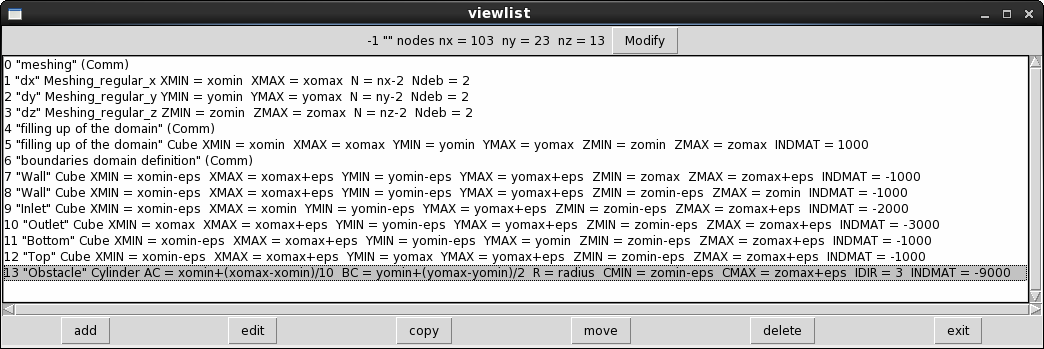
\includegraphics[width=1.1\textwidth]{xprepro_exo1_default_prep.png}
\end{figure}

If you open the file salome/exo1/model/defaut.prep which correspond to the previous picture, you must have some thing like:
\begin{alltt}
TAILLES 3 103 23 13 
RIEN 0 meshing
MAIL_X_REG 4 xomin xomax nx-2 2 dx
MAIL_Y_REG 4 yomin yomax ny-2 2 dy
MAIL_Z_REG 4 zomin zomax nz-2 2 dz
RIEN 0 filling up of the domain
PARALAX 7 xomin xomax yomin yomax zomin zomax 1000 filling up of the domain
RIEN 0 boundaries domain definition
PARALAX 7 xomin-eps xomax+eps yomin-eps yomax+eps zomax zomax+eps -1000 Wall
PARALAX 7 xomin-eps xomax+eps yomin-eps yomax+eps zomin-eps zomin -1000 Wall
PARALAX 7 xomin-eps xomin yomin-eps yomax+eps zomin-eps zomax+eps -2000 Inlet
PARALAX 7 xomax xomax+eps yomin-eps yomax+eps zomin-eps zomax+eps -3000 Outlet
PARALAX 7 xomin-eps xomax+eps yomin-eps yomin zomin-eps zomax+eps -1000 Bottom
PARALAX 7 xomin-eps xomax+eps yomax yomax+eps zomin-eps zomax+eps -1000 Top
CYLAX 7 xomin+(xomax-xomin)/10 yomin+(yomax-yomin)/2 radius zomin-eps zomax+eps 3 -9000 Obstacle
file maillage
        real xomin,xomax,yomin,yomax,zomin,zomax,eps,radius
C       Extremal sizes of the meshing
        xomin=0
        xomax=10
        yomin=0
        yomax=2
        zomin=0
        zomax=1
C       eps is useful for thickness of the blocks featuring boundaries
        eps=0.01
        radius=0.4
        XM(1)=xomin-eps
        XM(nx)=xomax+eps
        YM(1)=yomin-eps
        YM(ny)=yomax+eps
        ZM(1)=zomin-eps
        ZM(nz)=zomax+eps
\end{alltt}


which contain your salome/exo1/model/maillagedefaut file. If you open it, you must have:
\begin{alltt}
        real xomin,xomax,yomin,yomax,zomin,zomax,eps,radius
C       Extremal sizes of the meshing
        xomin=0
        xomax=10
        yomin=0
        yomax=2
        zomin=0
        zomax=1
C       eps is useful for thickness of the blocks featuring boundaries
        eps=0.01
        radius=0.4
        XM(1)=xomin-eps
        XM(nx)=xomax+eps
        YM(1)=yomin-eps
        YM(ny)=yomax+eps
        ZM(1)=zomin-eps
        ZM(nz)=zomax+eps
\end{alltt}


\newpage
\subsubsection{2D VDF mesh}
The "viewlist" file must look like:
\begin{figure}[h]
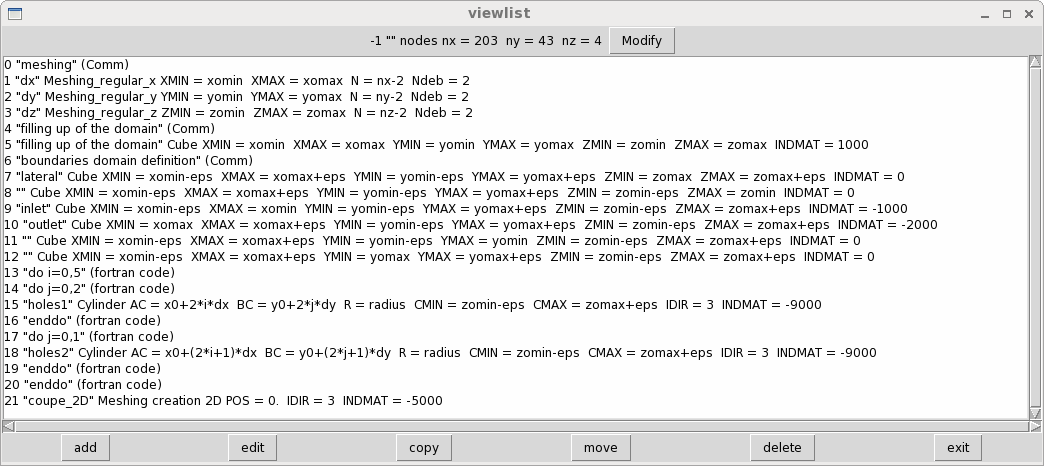
\includegraphics[width=1.1\textwidth]{xprepro_exo2_default_prep.png}
\end{figure}

If you open the file salome/exo2/model/defaut.prep which correspond to the previous picture, you must have some thing like:
\begin{alltt}
TAILLES 3 203 43 4 
RIEN 0 meshing
MAIL_X_REG 4 xomin xomax nx-2 2 dx
MAIL_Y_REG 4 yomin yomax ny-2 2 dy
MAIL_Z_REG 4 zomin zomax nz-2 2 dz
RIEN 0 filling up of the domain
PARALAX 7 xomin xomax yomin yomax zomin zomax 1000 filling up of the domain
RIEN 0 boundaries domain definition
PARALAX 7 xomin-eps xomax+eps yomin-eps yomax+eps zomax zomax+eps 0 lateral
PARALAX 7 xomin-eps xomax+eps yomin-eps yomax+eps zomin-eps zomin 0 
PARALAX 7 xomin-eps xomin yomin-eps yomax+eps zomin-eps zomax+eps -1000 inlet
PARALAX 7 xomax xomax+eps yomin-eps yomax+eps zomin-eps zomax+eps -2000 outlet
PARALAX 7 xomin-eps xomax+eps yomin-eps yomin zomin-eps zomax+eps 0 
PARALAX 7 xomin-eps xomax+eps yomax yomax+eps zomin-eps zomax+eps 0 
FORT 0 do i=0,5
FORT 0 do j=0,2
CYLAX 7 x0+2*i*dx y0+2*j*dy radius zomin-eps zomax+eps 3 -9000 holes1
FORT 0 enddo
FORT 0 do j=0,1
CYLAX 7 x0+(2*i+1)*dx y0+(2*j+1)*dy radius zomin-eps zomax+eps 3 -9000 holes2
FORT 0 enddo
FORT 0 enddo
COUPE2D 3 0. 3 -5000 coupe_2D
file maillage
        real xomin,xomax,yomin,yomax,zomin,zomax,eps,radius,dx,dy, x0, y0
C       Extremal sizes of the meshing
        xomin=0.
        xomax=10.
        yomin=0.
        yomax=2.
        zomin=0.
        zomax=0.01
C       eps is useful for thickness of the blocks featuring boundaries
        eps=0.0001
        radius=0.2
        dx=0.8
        dy=0.3
        x0=0.6
        y0=0.4
        XM(1)=xomin-eps
        XM(nx)=xomax+eps
        YM(1)=yomin-eps
        YM(ny)=yomax+eps
        ZM(1)=zomin-eps
        ZM(nz)=zomax+eps
\end{alltt}


which contain your salome/exo2/model/maillagedefaut file. If you open it, you must have:
\begin{alltt}
        real xomin,xomax,yomin,yomax,zomin,zomax,eps,radius,dx,dy, x0, y0
C       Extremal sizes of the meshing
        xomin=0.
        xomax=10.
        yomin=0.
        yomax=2.
        zomin=0.
        zomax=0.01
C       eps is useful for thickness of the blocks featuring boundaries
        eps=0.0001
        radius=0.2
        dx=0.8
        dy=0.3
        x0=0.6
        y0=0.4
        XM(1)=xomin-eps
        XM(nx)=xomax+eps
        YM(1)=yomin-eps
        YM(ny)=yomax+eps
        ZM(1)=zomin-eps
        ZM(nz)=zomax+eps
\end{alltt}




%%%%%%%%%%%%%%%%%%%%%%%%%%%%%%%%%%%%%%%%%%%%%%%%%%%%%%%%%%%%%%%%%%%%%%%%
\newpage
\section{Validation form}
\subsection{Canal.prm}
\begin{alltt}
Parameters \{
        Title "Check the debit_impose option of canal_perio keyword"
        Author "G.F."
        TestCase . std.data
        TestCase . debit.data
        TestCase . debit2.data
        TestCase . debit3.data
        TestCase . debit4.data
\}
Chapter \{
        Title "Comparison between flow rate specified by debit_impose option 
            and computed flow rate by the initial condition on velocity"
        Description "Data files differences:"
        Description include_text_file("diff_deb.out")
        Description "In the first data file, the flow rate will be 2 m3/s (Uo=1 m/s and S=2m). 
            In the second one, flow rate is 4 m3/s, and then will decrease to 2 m3/s."
        Figure \{
                dimension 2
                include_description_curves 0
                labely debit
                labelx time
                Curve \{
                        fichier std_pb_Debit.out
                        legend std
                        style lines
                \}
                Curve \{
                        fichier debit_pb_Debit.out
                        legend debit_impose
                        style lines
                \}
        \}
\}
Chapter \{
        
        Title "Initial velocity is inclined into 2 directions, with a vertical flow 
            rate which should be 0."
        Description "When converged, the velocity profile reaches horizontality."
        Description
        Visu \{
                blackVector debit2.lata dom VITESSE SOM
                # operator_to_all no_databaseinfo
                cycles 0 -1
                width 7.5cm
                nb_img_without_newline 2 
        \}
\}
Chapter \{
        
        Title "Initial velocity is inclined into 2 directions, with a vertical flow rate 
            which should be 0."
        Description "When converged, the velocity profile reaches horizontality to 4 
            (due to the porosity) ."
        Description
        Visu \{
                Vector debit3.lata dom VITESSE SOM
                # operator_to_all no_databaseinfo
                cycles 0 -1
                width 7.5cm
                nb_img_without_newline 2 
        \}
\}
{\bf{
Chapter \{
        Title "Additional information"
        Visu \{
                Title "Mesh visualization"
                Mesh debit.lata dom blue
                Width 9cm
        \}
        Figure \{
                Title "Residus evolution"
                LabelX "Time (s)"
                LabelY "Residu"
                LogX
                LogY
                Width 9cm
                Include_description_curves 0
                Curve \{
                        legend "Test case debit.data"
                        file debit.dt_ev
                        columns $1 $4
                        style lines
                \}
                Curve \{
                        legend "Test case debit2.data"
                        file debit2.dt_ev
                        columns $1 $4
                        style lines
                \}
                Curve \{
                        legend "Test case debit3.data"
                        file debit3.dt_ev
                        columns $1 $4
                        style lines
                \}
                Curve \{
                        legend "Test case debit4.data"
                        file debit4.dt_ev
                        columns $1 $4
                        style lines
                \}
                Curve \{
                        legend "Test case std.data"
                        file std.dt_ev
                        columns $1 $4
                        style lines
                \}
        \}
        Visu \{
                Title "Visualization of the pressure field at last time"
                Description "Visualization of the pressure field at last time of the test case debit2.data."
                Pseudocolor debit2.lata dom PRESSION ELEM
                Cycles -1
                Width 7.5cm
        \}
        Visu \{
                Title "Vizualization of velocity field at last time, test case std"
                Pseudocolor std.lata dom_dual_magnitude VITESSE FACES
                Cycles -1
                Width 7.5cm
        \}
        Table \{
                Title "Number of cells and last time results"
                Nb_columns 5
                Label "std" | "debit" | "debit2" | "debit3" | "debit4"
                Line \{
                        legend "cell numbers"
                        file nbcells.dat
                        columns $1 $2 $3 $4 $5
                \}
                Line \{
                        legend "last time (s)"
                        file lastime.dat
                        columns $1 $2 $3 $4 $5
                \}
        \}
}}
\}
\end{alltt}

\subsection{prepare}
\begin{alltt}
#!/bin/sh
sed "s/champ_uniforme 2 1. 0./ champ_uniforme 2 2 0./;
    s/bord periox/ bord periox debit_impose 2./" std.data >  debit.data
diff std.data debit.data > diff_deb.out
sed "s/paroi_fixe/periodique/;
    s/champ_uniforme 2 1. 0../ champ_uniforme 2 2. 1./;
    s/bord periox/ bord periox debit_impose 2./;
    s/# balise #/sources \{ Canal_perio \{  bord haut debit_impose 0 \} \}/" std.data > debit2.data
diff std.data debit2.data | grep -v balise > diff_deb2.out
sed "s/Discretize pb dis/Discretize pb dis Porosites_champ pb champ_uniforme 1 0.25/;
    s/Trianguler_Fin dom/Trianguler_Fin dom transformer dom x+y y/" debit2.data > debit3.data 
diff debit2.data debit3.data | grep -v balise > diff_deb3.out
{\bf{sed "s/champ_uniforme 2 1. 0./ champ_uniforme 2 0 0./;
    s/bord periox/ bord periox debit_impose 2./" std.data >  debit4.data
diff std.data debit4.data  | grep -v balise > diff_deb4.out }}
\end{alltt}

\subsection{post\_run}
\begin{alltt}
#!/bin/sh
nb1=`grep "Total number of elements" std.err    | awk '\{print $NF\}'`
nb2=`grep "Total number of elements" debit.err  | awk '\{print $NF\}'`
nb3=`grep "Total number of elements" debit2.err | awk '\{print $NF\}'`
nb4=`grep "Total number of elements" debit3.err | awk '\{print $NF\}'`
{\bf{nb5=`grep "Total number of elements" debit4.err | awk '\{print $NF\}'`}}
{\bf{echo $nb1 $nb2 $nb3 $nb4 $nb5 > nbcells.dat}}
tp1=`grep "Backup of the field" std.err    | awk '\{print $NF\}' | head -n 1`
tp2=`grep "Backup of the field" debit.err  | awk '\{print $NF\}' | head -n 1`
tp3=`grep "Backup of the field" debit2.err | awk '\{print $NF\}' | head -n 1`
tp4=`grep "Backup of the field" debit3.err | awk '\{print $NF\}' | head -n 1`
{\bf{tp5=`grep "Backup of the field" debit4.err | awk '\{print $NF\}' | head -n 1`}}
{\bf{echo $tp1 $tp2 $tp3 $tp4 $tp5 > lastime.dat}}
\end{alltt}



%%%%%%%%%%%%%%%%%%%%%%%%%%%%%%%%%%%%%%%%%%%%%%%%%%%%%%%%%%%%%%%%%%%%%%%%
\end{document}

